\chapter{Обобщенная модель Изинга на квадратной решетке}\label{ch:ch4}

Первой работой по обобщению модели Изинга на несколько трансляций решетки была статья Утиямы~\cite{utiyama1951} на примере шахматной решетки, в которой все черные квадраты замещаются специальными вставками~(рисунок~\ref{utiyamaGen}). В случае, когда $n=0$, что означает всего один квадрат в качестве вставки со взаимодействиями $J, J_1$ и $J_0$, можно получить квадратную необобщенную, треугольную и гексагональную решетки. Положив $n=1$, получим решетку кагоме (в качестве вставки два квадрата со взаимодействиями $J, J_0, J_1, J_2, J_3$) и устремив $J_1$ к нулю (рисунок~\ref{toKagome}). Таким образом, обобщение модели Изинга при больших $n$ дает колоссальное количество новых еще неисследованных решеток.

 \begin{figure}[h]
 	\center{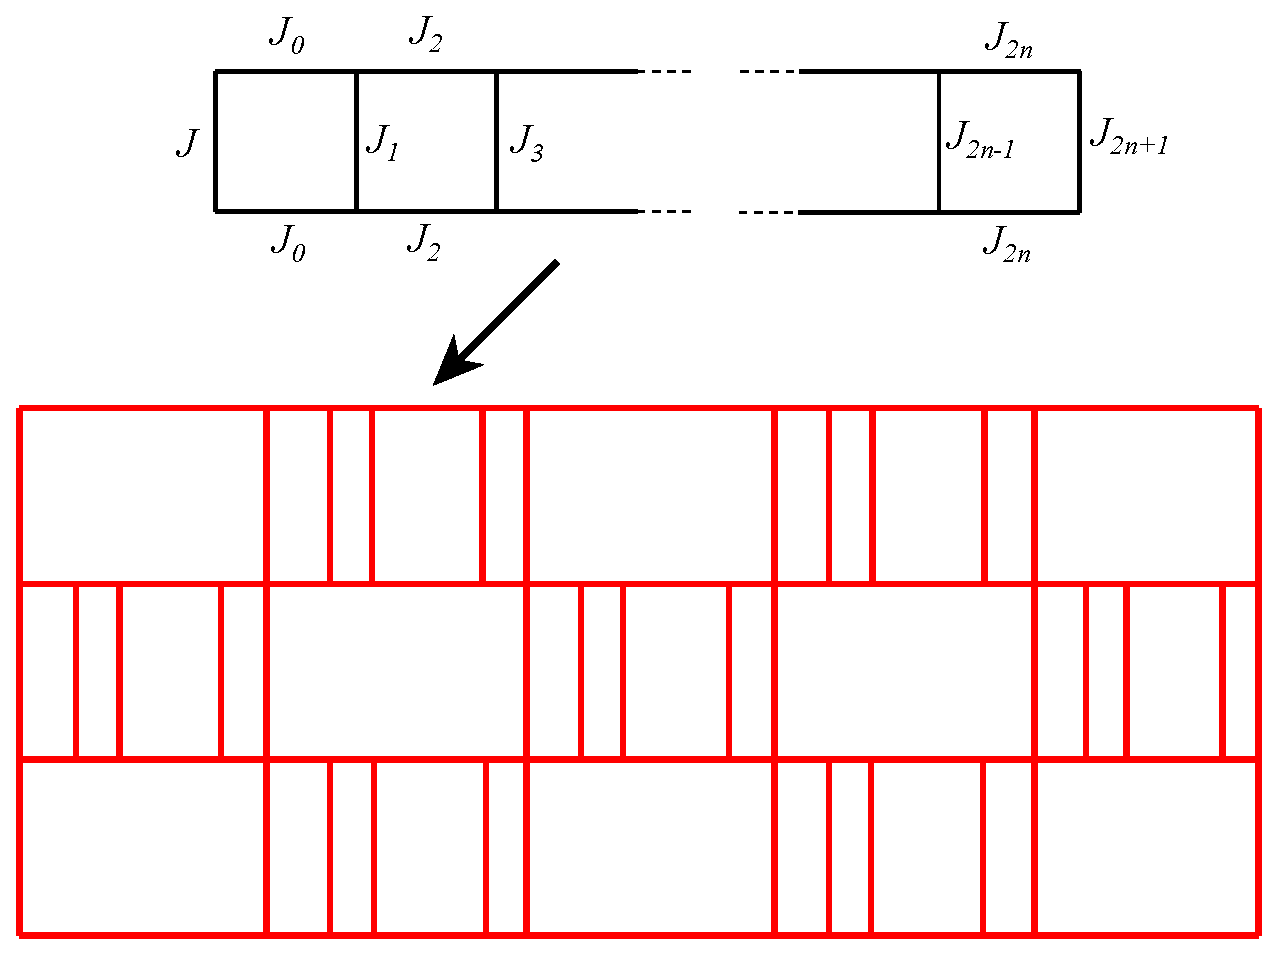
\includegraphics[width=0.6\linewidth]{part4/utiyamaGen.eps}}
 	\caption{Обобщение модели Изинга, предложенное Утиямой, на шахматной решетке}
 	\label{utiyamaGen}
 \end{figure}

 \begin{figure}[h]
 	\begin{minipage}{0.45\linewidth}
 		\center{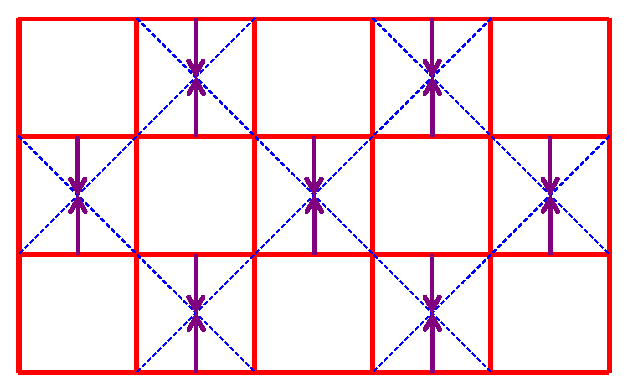
\includegraphics[width=1\linewidth]{part4/toKagome1.eps} \\ а)}
 	\end{minipage}
 	\hfill
 	\begin{minipage}{0.45\linewidth}
 		\center{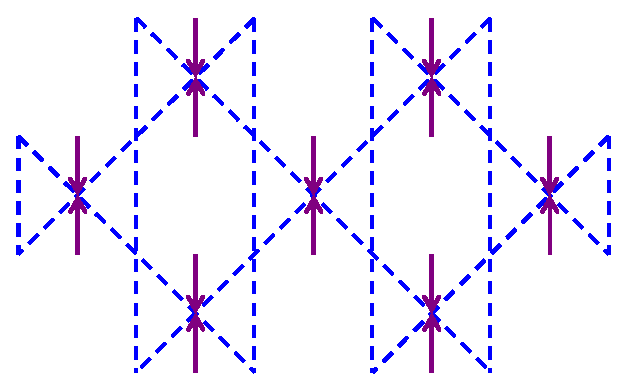
\includegraphics[width=1\linewidth]{part4/toKagome2.eps} \\ б)}
 	\end{minipage}
 	\caption{Переход от решетки Утиямы ($n=1$) к решетке кагоме: а) Решетка Утиямы с одной вертикальной чертой при $J_1 \rightarrow 0$, б) Решетка кагоме}
 	\label{toKagome}
 \end{figure}

Следующими работами по обобщению модели Изинга стали статьи Сиози и Найя~\cite{syozi1960} (см. также~\cite{siozi_domb1972}). В этих работах авторы приводят точное аналитическое решение обобщенной модели Изинга на квадратной решетке с двумя трансляциями в горизонтальном ($J_{2}, J_{4}$) и вертикальном ($J_{1}, J_{3}$) направлениях~(рисунок~\ref{genSquare}). Синими прямыми указаны связи между соседними спинами по горизонтальному направлению с обменным взаимодействием $J_1$, синими пунктирными линиями по горизонтальному направлению  --- $J_3$, красными прямыми линиями по вертикальному направлению --- $J_2$, красными пунктирными линиями по вертикальному направлению --- $J_4$. Обратим внимание, что помимо точного решения исследований каких-либо термодинамических и фрустрационных свойств не проводилось.

Главным преимуществом обобщенной решетки является то, что из структуры такого типа обобщения можно получать различные виды других решеток с помощью предельных переходов. Например, при $J_1 = J_3$ и $J_2 = J_4$ решетка сводится к обычной квадратной решетке, решение которой рассмотрено в Главе~\ref{ch:ch1}. Так же может быть осуществлен переход к гексагональной решетке. Для этого необходимо устремить к нулю одно из четырех обменных взаимодействий, например, $J_4 \rightarrow 0$. Получаемая таким образом решетка типа \guillemotleft кирпичная кладка\guillemotright$ $ (brick-wall lattice) %, показанная на рисунке~\ref{toHex}, 
топологически эквивалентна гексагональной решетке.

 \begin{figure}[h]
 	\center{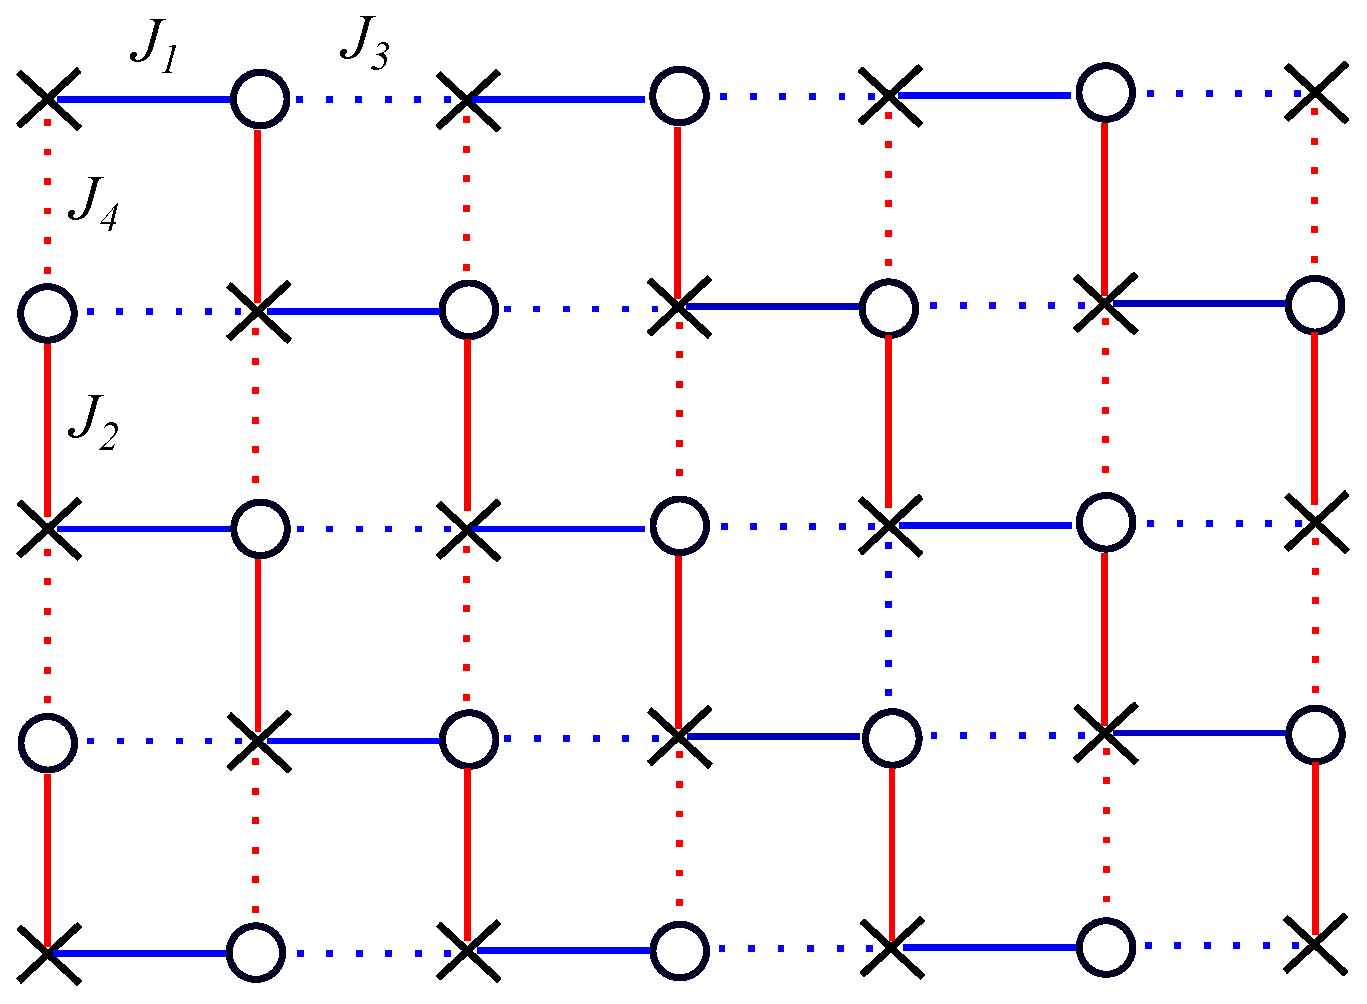
\includegraphics[width=0.6\linewidth]{part4/genSquare.eps}}
 	\caption{Обобщенная квадратная решетка}
 	\label{genSquare}
 \end{figure}
 
В случае же перехода к треугольной решетке, одно из четырех обменных взаимодействий обобщенной модели устремляется в бесконечность, например, $J_1 \rightarrow \infty$.%, (см. рисунок~\ref{toTriag}).

Очевидно, что данные варианты обобщения, введенные на квадратной решетке Утиямой, Сиози и Найя, могут быть применены и к другим планарным решеткам с известными точными решениями (треугольная~\cite{wannier1950}, гексагональная~\cite{houtapell1950}, кагоме~\cite{kano_naya1953}). В результате, всевозможными вариантами предельных переходов осуществляется получение множества самых разнообразных видов еще неизученных решеток.

% \begin{figure}[h]
% 	\center{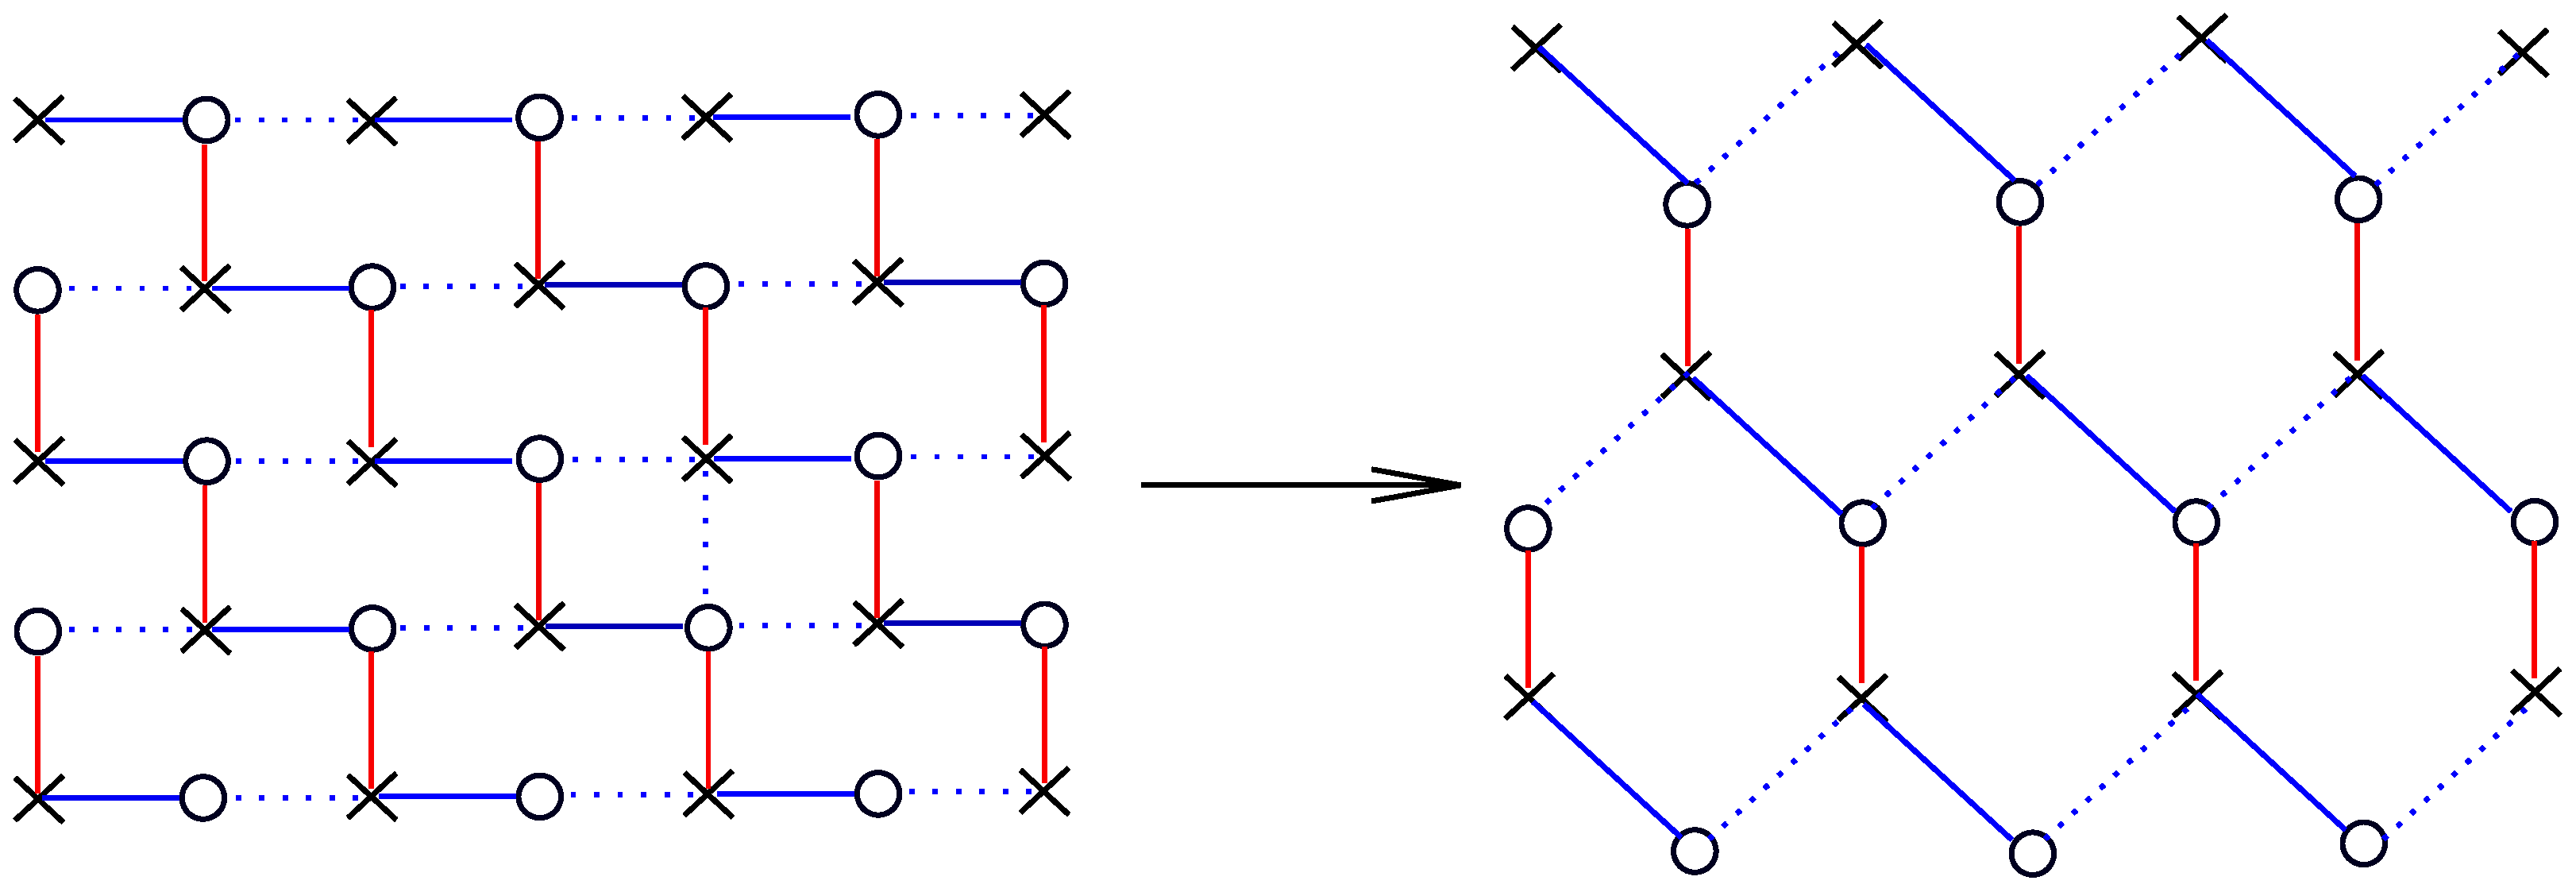
\includegraphics[width=1\linewidth]{part4/toHex.eps}}
% 	\caption{При $J_4 = 0$ обобщенная квадратная решетка превращается в так называемую кирпичную кладку, которая топологически эквивалентна гексагональной решетке}
% 	\label{toHex}
% \end{figure}
%
% \begin{figure}[h]
% 	\center{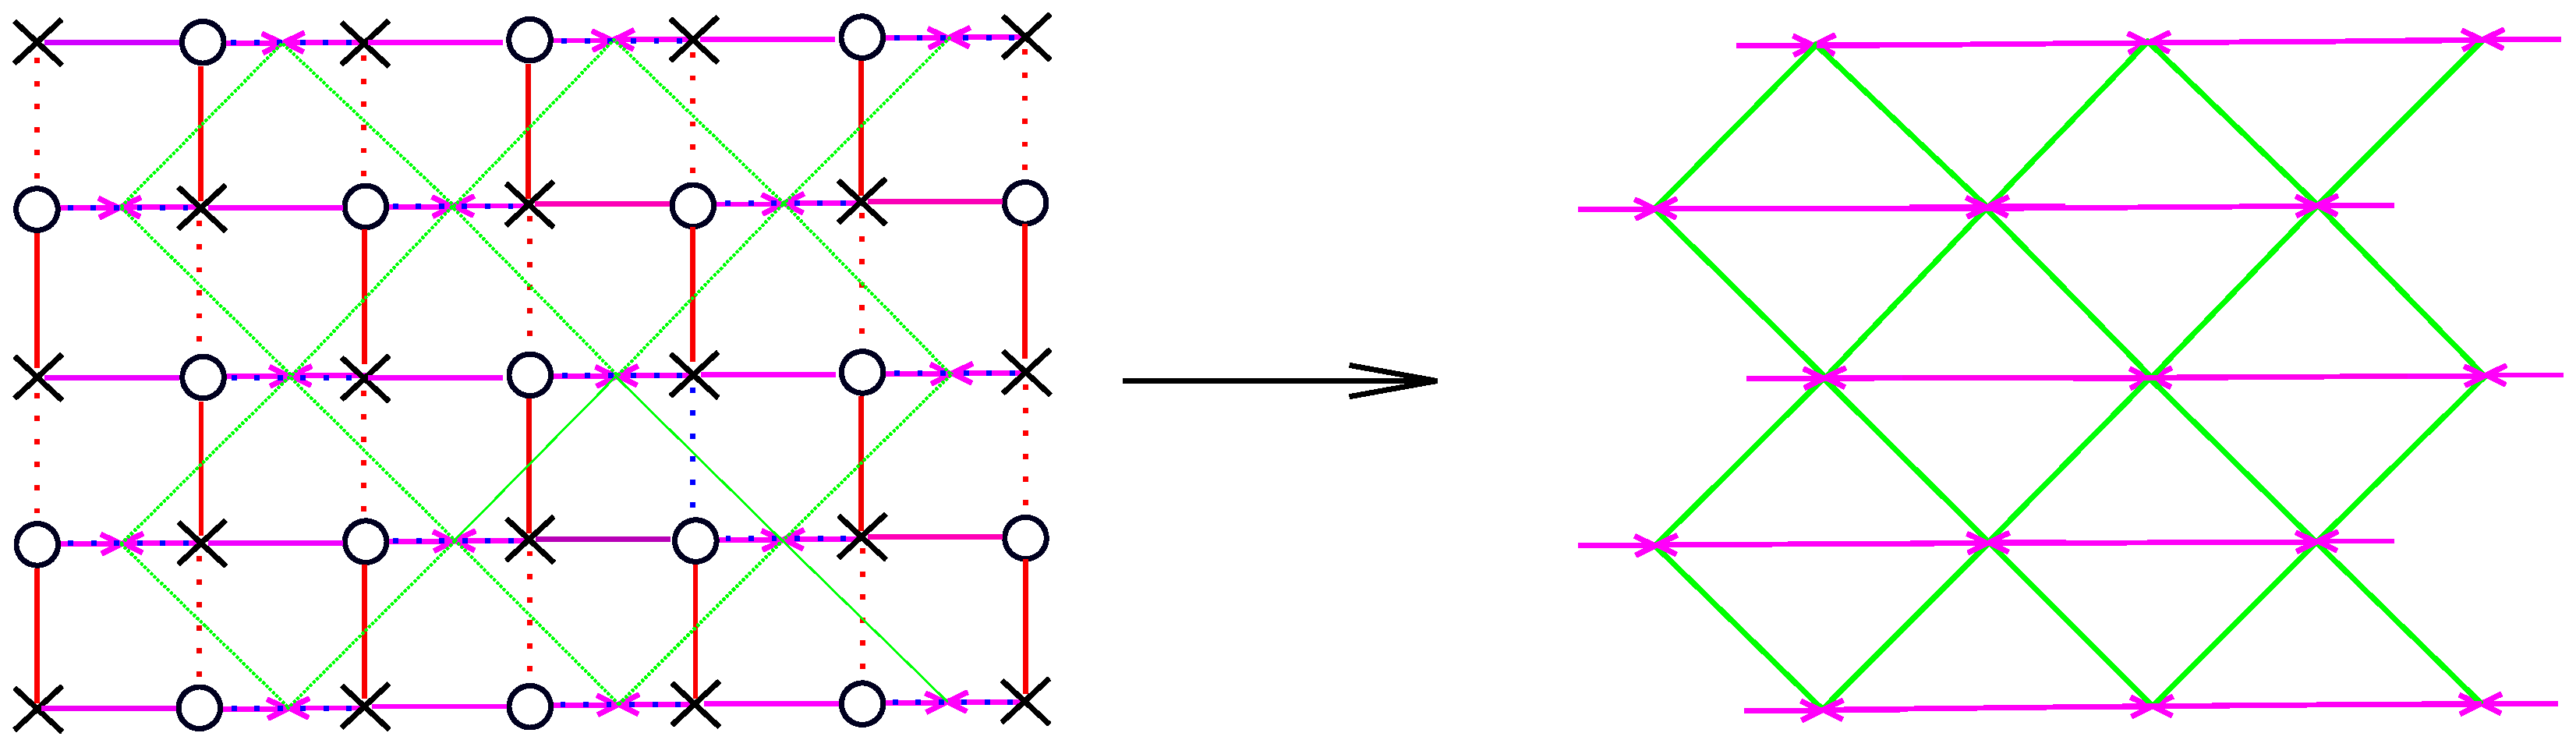
\includegraphics[width=1\linewidth]{part4/toTriag.eps}}
% 	\caption{Переход от обобщенной квадратной решетки к треугольной решетке при $J_1 \rightarrow \infty$}
% 	\label{toTriag}
% \end{figure}

В настоящей кандидатской диссертации рассматривается модель Изинга на обобщенной квадратной решетке (рисунок \ref{genSquare}), с последующим изучением ее термодинамических и фрустрационных свойств. 


\section{Точное решение обобщенной модели Изинга на квадратной решетке}

Получим точное аналитическое решение обобщенной модели Изинга на квадратной решетке комбинаторным методом Вдовиченко--Фейнмана.

Статсумму приведенной решетки можно представить следующим образом 
\begin{multline}
Z_{N} = \sum_{\{\sigma\}} \exp{\bigg[ K_1 \sum_{\substack{i = 1,3,\dots \\ j = 2,4,\dots}} \sigma_i \sigma_j + K_2 \sum_{\substack{i = 2,4,\dots \\ k = 3,5,\dots}} \sigma_i \sigma_k + }\\{ +  K_3 \sum_{\substack{i = 2,4,\dots \\ j = 3,5,\dots}} \sigma_i \sigma_j + K_4 \sum_{\substack{i = 1,3,\dots \\ k = 2,4,\dots}} \sigma_i \sigma_k\bigg]},
\end{multline}
где первая и третья суммы идут по половинам спинов в горизонтальном направлении,  а вторая и четвертая суммы идут по половинам спинов в вертикальном направлении, так что
\begin{equation*}
K_1 = \frac{J_1}{T}; \;\;\;\;\;\; K_2 = \frac{J_2}{T};\;\;\;\;\;\; K_3 = \frac{J_3}{T};\;\;\;\;\;\;K_4 = \frac{J_4}{T}.
\end{equation*}

Перепишем статсумму в виде
\begin{align}
&Z_{N} = (\ch K_1 \ch K_2 \ch K_3 \ch K_4)^N S, \nonumber \\
&S = \sum_{\{\sigma\}} \prod_{\substack{i = 1,3,\dots \\ j = 2,4,\dots}} (1 + v \sigma_i \sigma_j) \prod_{\substack{i = 2,4,\dots \\ k = 3,5,\dots}} (1 + u \sigma_i \sigma_k) \times \nonumber\\&\;\;\;\;\;\;\;\;\; \times \prod_{\substack{i = 2,4,\dots \\ j = 3,5,\dots}} (1 + w \sigma_i \sigma_j) \prod_{\substack{i = 1,3,\dots \\ k = 2,4,\dots}} (1 + t \sigma_i \sigma_k).
\label{z} 
\end{align}

Здесь $v = \th K_1$, $u = \th K_2$, $w = \th K_3$, $t = \th K_4$, а $N = L^2$ --- число спинов в решетке. Величина $S$ является полиномом от $v$, $u$, $w$ и $t$, в котором коэффициент $g_{nmlk}$ при $v^n u^m w^l t^k$ равен количеству способов построения замкнутых многоугольников, при которых общее количество горизонтальных связей равно $n+l$, а общее количество вертикальных связей равно $m+k$.

В статье Вдовиченко~\cite{vdovichenko1965_1} показано, что для модели Изинга на обычной квадратной решетки величина $g_{nm}$ может быть представлена ​​в виде суммы по замкнутым циклам, причем каждый цикл берется с множителем $(-1)^s$, где $s$ --- количество самопересечений замкнутого многоугольника. Наш случай ни сколько не отличается от обычного, за исключением того, что на обобщенной квадратной решетке встречаются два вида узлов (рисунок \ref{point}) (см. статьи~\cite{vaks1966, chikyu1987}). У узла, помеченного крестом (рисунок \ref{point}a), связь между соседним верхним узлом с обменным взаимодействием $J_2$, между соседним нижним узлом --- $J_4$, между соседним левым узлом --- $J_3$, между соседним левым узлом --- $J_1$. У узла, обозначенного кружком (рисунок \ref{point}б), наоборот: связь между соседним верхним узлом с обменным взаимодействием $J_4$, между соседним нижним узлом --- $J_2$, между соседним левым узлом --- $J_1$, между соседним левым узлом --- $J_3$. 

 \begin{figure}[h]
 	\begin{minipage}[h]{0.4\linewidth}
 		\center{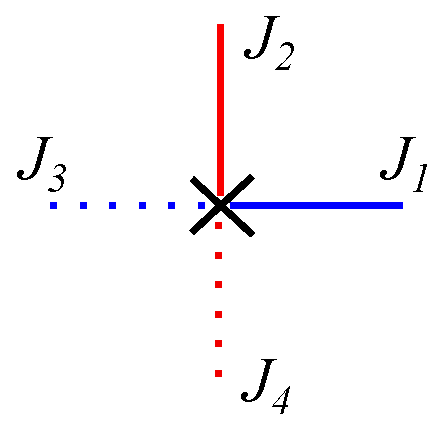
\includegraphics[width=0.7\linewidth]{part4/point1.eps} \\ а)}
 	\end{minipage}
 	\hfill
 	\begin{minipage}[h]{0.4\linewidth}
 		\center{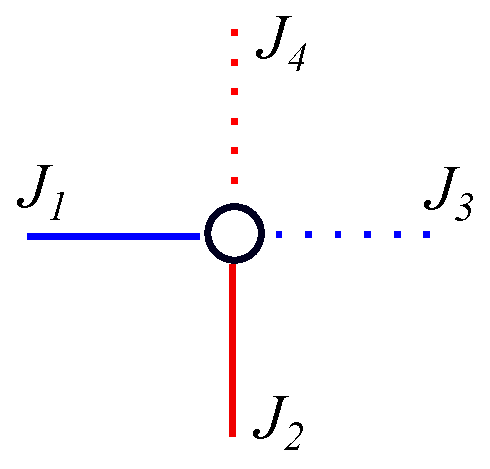
\includegraphics[width=0.7\linewidth]{part4/point2.eps} \\ б)}
 	\end{minipage}
 	\caption{Два вида узлов на обобщенной квадратной решетке}
 	\label{point}
 \end{figure}

В связи с этим, в отличие от обычной квадратной решетки, имеем 8 различных направлений на обобщенной квадратной решетке (рисунок \ref{directionGen}): 4 направления из узла , обозначенного кружком (вверх, вниз, влево, вправо) и 4 направления из узла, обозначенного крестом (вверх, вниз, влево, вправо).

 \begin{figure}[h]
 	\center{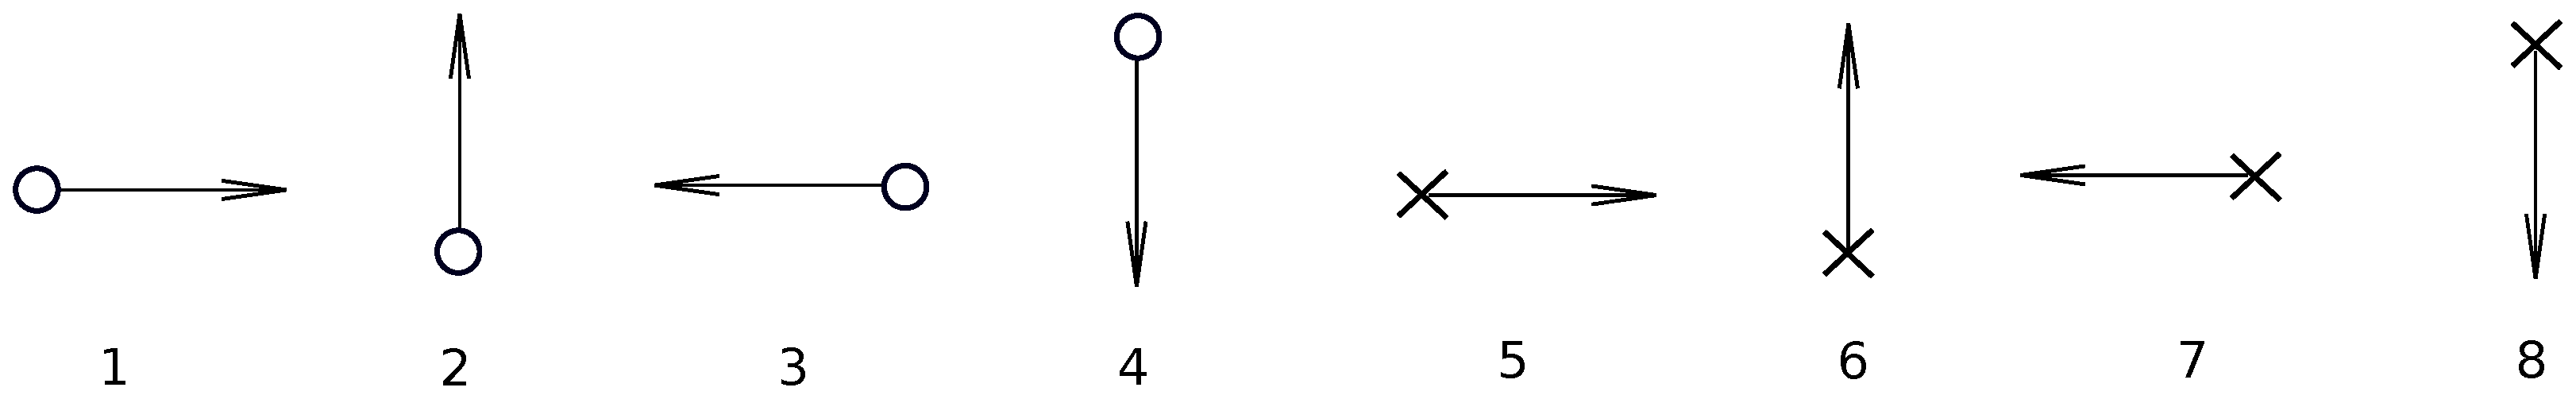
\includegraphics[width=0.9\linewidth]{part4/directionGen.eps}}
 	\caption{Возможные направления на обобщенной квадратной решетке}
 	\label{directionGen}
 \end{figure}

Так же как и в случае обычной квадратной решетки, введем матрицу коэффициентов $\Lambda$, рекурсивные уравнения можно записать в виде
\begin{equation}
W_{r+1}(i, j, \mu) = \sum_{i^{'},\; j^{'},\; \mu^{'}} \Lambda (ij\mu\; |\; i^{'}j^{'}\mu^{'}) W_{r} (i^{'}, j^{'}, \mu^{'}),
\end{equation}

Поскольку существует восемь возможных направлений для движения по решетке, $\Lambda$ представляет собой матрицу $8 \times 8$ с индексами $\mu^{'}$ и $\mu$, графическая интерпретация которой показана на рисунке \ref{matrixGen}. 

 \begin{figure}[h]
 	\center{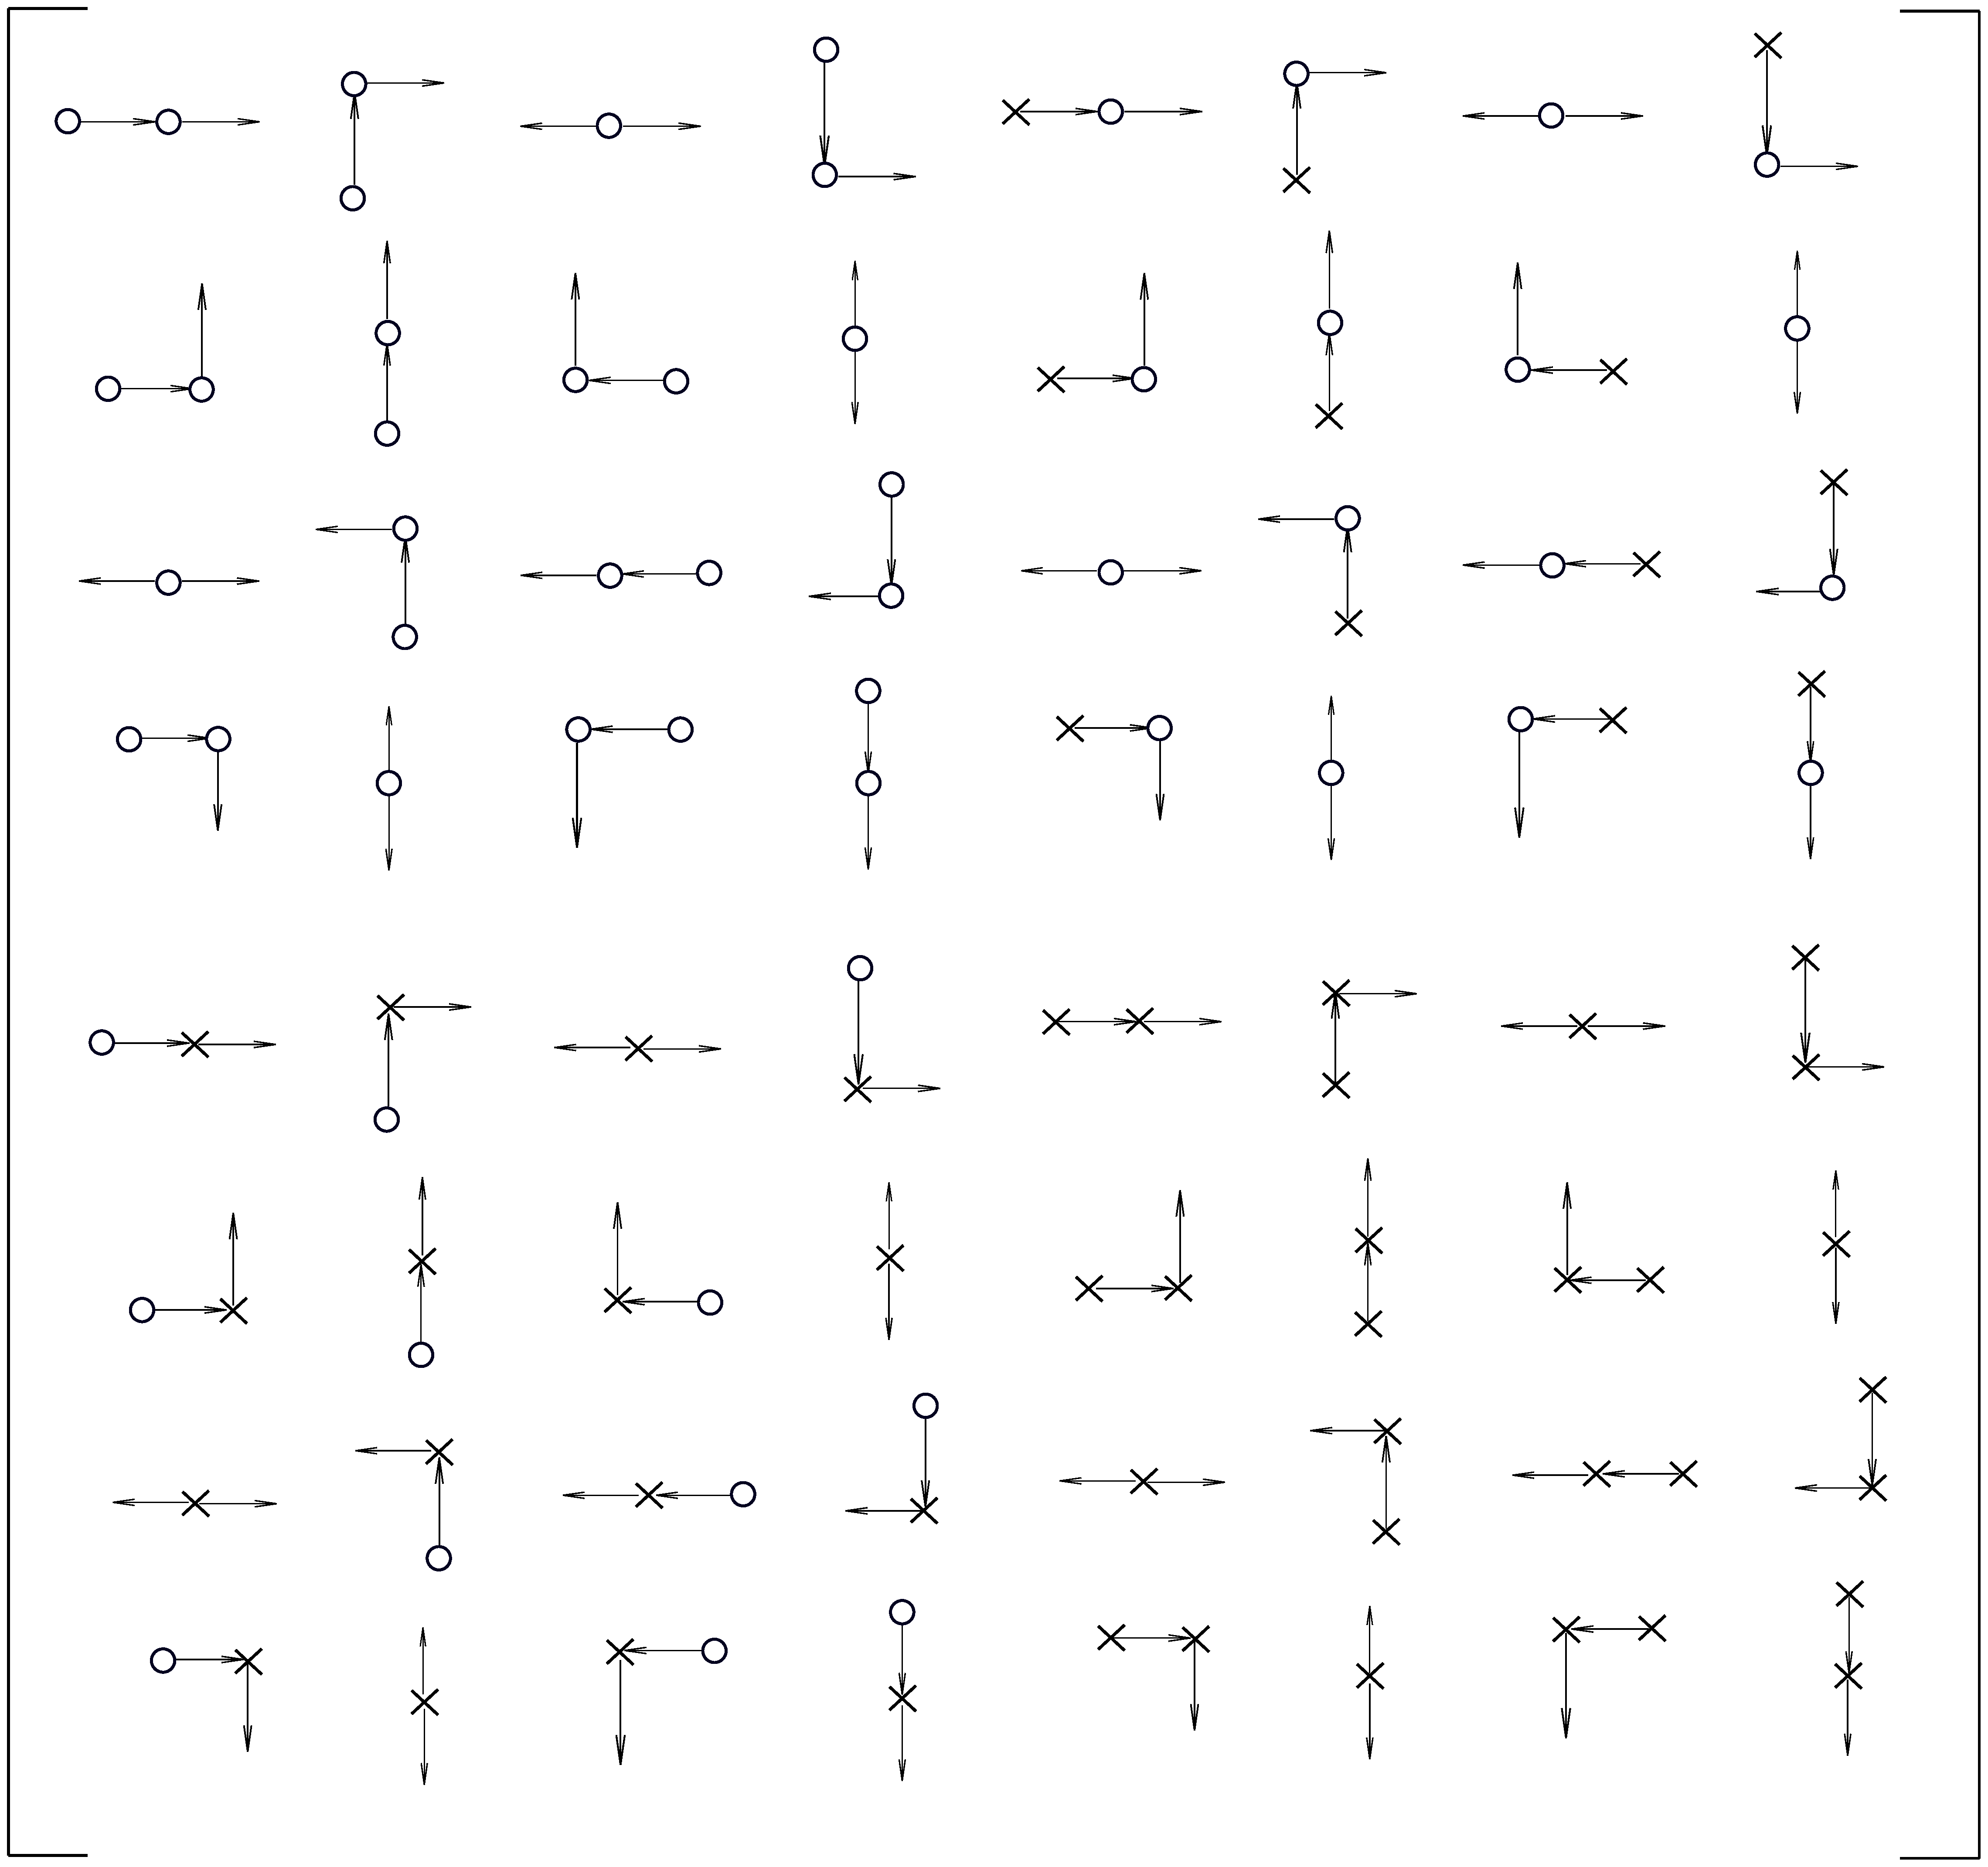
\includegraphics[width=0.9\linewidth]{part4/matrixGen.eps}}
 	\caption{Матричные элементы $\Lambda$}
 	\label{matrixGen}
 \end{figure}

Однако, стоит заметить, что оказывается матрица $\Lambda$ имеет более простой вид, отличный от представленного на рисунке  \ref{matrixGen}. Так как у нас не существует направлений движения, при котором из узла, обозначенного кружком, мы бы попадали в такой же узел и, также, у нас не существует направлений движения, при котором из узла, обозначенного крестом, мы бы попадали в похожий узел, поэтому все эти матричные элементы будут равны нулю.

Принимая это во внимание, запишем окончательный вид матрицы коэффициентов $\Lambda$ для обобщенной квадратной решетки в следующем виде

\begin{multline}
\Lambda (p, q, \mu\; |\; p, q, \mu^{'}) = \\ =
\begin{pmatrix}
0 \!\!\!& 0 \!\!\!& 0 \!\!\!& 0\!\!\! & v \epsilon^{-p} \!\!\!& u \alpha^{-1} \epsilon^{-q} \!\!\!& 0 \!\!\!& t \alpha \epsilon^{q} \!\!\! \\
0 \!\!\!& 0 \!\!\!& 0 \!\!\!& 0 \!\!\!& v \alpha \epsilon^{-p}\!\!\! & u \epsilon^{-q}\!\!\! & w \alpha^{-1} \epsilon^{p}\!\!\! & 0\!\!\! \\
0 \!\!\!& 0 \!\!\!& 0 \!\!\!& 0\!\!\! & 0\!\!\! & u \alpha \epsilon^{-q} \!\!\!& w \epsilon^{p} \!\!\!& t \alpha^{-1} \epsilon^{q}\!\!\!  \\
0 \!\!\!& 0 \!\!\!& 0 \!\!\!& 0\!\!\! & v \alpha^{-1} \epsilon^{-p}\!\!\! & 0 \!\!\!& w \alpha \epsilon^{p} \!\!\!& t \epsilon^{q}\!\!\!  \\
w \epsilon^{-p} \!\!\!& t \alpha^{-1} \epsilon^{-q} \!\!\!& 0\!\!\! & u \alpha \epsilon^{q}\!\!\! & 0\!\!\! & 0\!\!\! & 0\!\!\! & 0\!\!\!  \\
w \alpha \epsilon^{-p}\!\!\! & t \epsilon^{-q} \!\!\!& v \alpha^{-1} \epsilon^{p}\!\!\! & 0 \!\!\!& 0\!\!\! & 0\!\!\! & 0\!\!\! & 0\!\!\! \\
0 \!\!\!& t \alpha \epsilon^{-q}\!\!\! & v \epsilon^{p} \!\!\!& u \alpha^{-1} \epsilon^{q}\!\!\! & 0 \!\!\!& 0\!\!\! & 0\!\!\! & 0 \!\!\! \\
w \alpha^{-1} \epsilon^{-p}\!\!\! & 0\!\!\! & v \alpha \epsilon^{p}\!\!\! & u \epsilon^{q} \!\!\!& 0\!\!\! & 0\!\!\! & 0 \!\!\!& 0 \!\!\!
\end{pmatrix},
\end{multline}
где $\epsilon = e^{2\pi i/L}$ и $\alpha = e^{i\pi/4}$.

Следуя алгоритму комбинаторного метода и производя несложные вычисления, имеем точное аналитическое решение обобщенной модели Изинга на квадратной решетке 
\begin{multline}
\ln \frac{\lambda_g}{2} = \frac{1}{16 \pi^2} \int_{0}^{2\pi} \int_{0}^{2\pi} \ln \bigg[\frac{1}{2} \bigg( \ch 2K_1 \ch 2K_2 \ch 2K_3 \ch 2K_4 + \\
+ \sh 2K_1 \sh 2K_2 \sh 2K_3 \sh 2K_4 + 1 - \sh 2K_1 \sh 2K_3 \cos (\omega_1 + \omega_2)  - \\ - \sh 2 K_2 \sh 2 K_4 \cos (\omega_1 - \omega_2)  - (\sh 2 K_1 \sh 2 K_4 + \sh 2 K_2 \sh 2 K_3) \cos \omega_1  - \\ - (\sh 2 K_1 \sh 2 K_2 + \sh 2 K_3 \sh 2 K_4) \cos \omega_2 \bigg) \bigg] d\omega_1 d\omega_2,
\end{multline}
где $K_1 = J_1/T$, $K_2 = J_2/T$, $K_3 = J_3/T$, $K_4 = J_4/T$. 

После чего, термодинамические параметры системы, такие как свободная энергия, энтропия и теплоемкость, находятся без труда уже по известным формулам термодинамики \eqref{eq:1.13}, \eqref{eq:1.15}, \eqref{eq:1.16} соответственно.

\section{Термодинамические и фрустрационные особенности обобщенной модели Изинга на квадратной решетке}

Обобщенная модель Изинга, в отличие от обычной, привлекательна тем, что позволяет задавать различные обменные взаимодействия между парами спинов, не только по значению, но и по знаку. В данной работе имеется 4 обменных взаимодействия: $J_1$, $J_2$, $J_3$ и $J_4$. Это означает, что существует $2^4 = 16$ различных комбинаций задания знаков между спинами. А вариантов обменных взаимодействий с различными значениями еще больше... Поэтому, изначально рассмотрены обменные взаимодействия только с различными знаками, положив взаимодействия по модулю равными единице, $|J_1| = |J_2| = |J_3| = |J_4| = 1$. Здесь и как и ранее в тексте, обменное взаимодействие, отмеченное знаком "$+$" ферромагнитным, а знаком "$-$" антиферромагнитным.

\begin{align*}
	&1) +\;+\;+\;+\;, \qquad   5) +\;-\;+\;+\;, \qquad	 \;\;9) -\;+\;+\;+\;, \qquad	 13) -\;-\;+\;+\;, \\
	&2) +\;+\;+\;-\;, \qquad  6) +\;-\;+\;-\;, \qquad	 10) -\;+\;+\;-\;, \qquad	 14) -\;-\;+\;-\;, \\
	&3) +\;+\;-\;+\;, \qquad  7) +\;-\;-\;+\;, \qquad  11) -\;+\;-\;+\;, \qquad	 15) -\;-\;-\;+\;, \\
	&4) +\;+\;-\;-\;, \qquad  8) +\;-\;-\;-\;, \qquad	 12) -\;+\;-\;-\;, \qquad	 16) -\;-\;-\;-\;.
\end{align*}

Случаи, отмеченные номерами $1), 16)$ вместе с $|J_1| = |J_2| = |J_3| = |J_4| = 1$ очевидно дают обычную (необобщенную) квадратную решетку~\cite{onsager1941}, с температурными зависимостями энтропии и теплоемкостью, указанных на рисунке~\ref{SimpleSquareLattice}. Те же температурные зависимости дают случаи, отмеченные номерами $4), 6), 7), 10), 11)$ и $13)$. Эти случаи не дают фрустрационных состояний~\cite{toulouse1977, vannimenus1977}, а все потому что, спины на квадратной решетке можно расположить таким образом, чтобы удовлетворить всем обменным взаимодействиям.

\begin{figure}[h]
	\begin{minipage}[h]{0.5\linewidth}
		\center{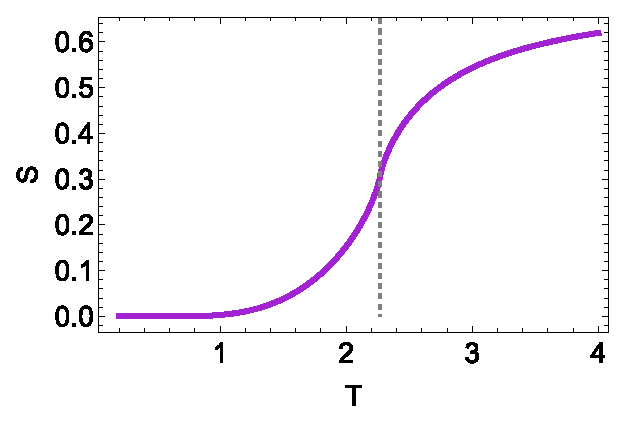
\includegraphics[width=1\linewidth]{part4/squareLatticeS.eps} \\ а)}
	\end{minipage}
	\hfill
	\begin{minipage}[h]{0.5\linewidth}
		\center{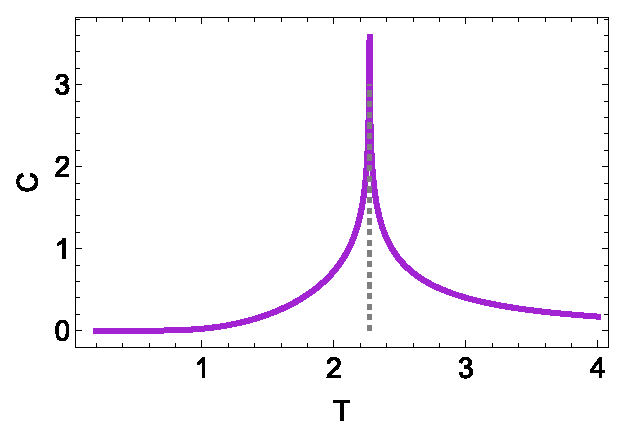
\includegraphics[width=1\linewidth]{part4/squareLatticeC.eps} \\ б)}
	\end{minipage}
	\caption{Температурные зависимости обычной квадратной решетки: а) энтропия, б) теплоемкость. Пунктирной линией обозначена температура перехода квадратной решетки: $T_c = 2/(\ln(1+\sqrt{2}))\approx 2.2692$.}
	\label{SimpleSquareLattice}
\end{figure}

Фрустрацию можно получить, если положить одно из взаимодействий антиферромагнитным, а остальные будут ферромагнитными (или, наоборот, одно из взаимодействий ферромагнитно, а другие антиферромагнитны). И неважно какое взаимодействие будет антиферромагнитным (или, наоборот, ферромагнитным). К таким вариантам относятся оставшиеся случаи из списка: $2), 3), 5), 8), 9), 12), 14)$ и $15)$.

\begin{figure}[h]
	\begin{minipage}[h]{0.5\linewidth}
		\center{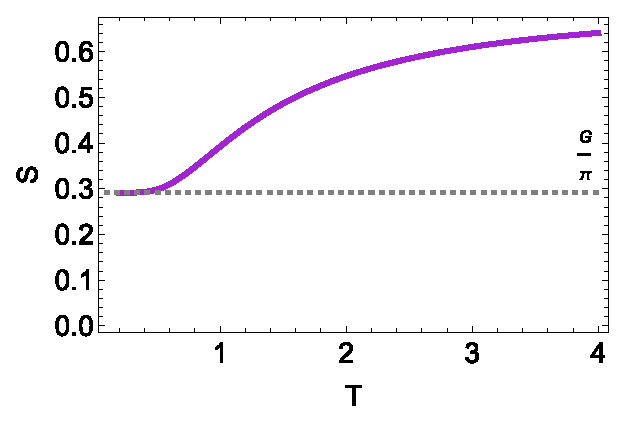
\includegraphics[width=1\linewidth]{part4/catalanS.eps} \\ а)}
	\end{minipage}
	\hfill
	\begin{minipage}[h]{0.5\linewidth}
		\center{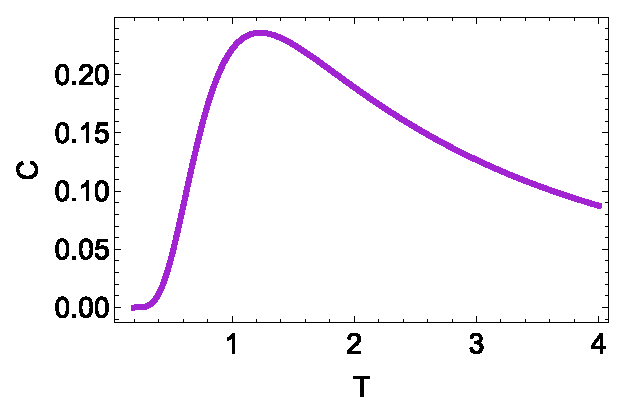
\includegraphics[width=1\linewidth]{part4/catalanC.eps} \\ б)}
	\end{minipage}
	\caption{Температурные зависимости обобщенной квадратной решетки c одним ферромагнитным (или антиферромагнитным) взаимодействием и тремя антиферромагнитными (или ферромагнитными) взаимодействиями: а) энтропия, б) теплоемкость. Пунктирной линией обозначена нуль-температурная энтропия: $S_{T\rightarrow 0} = G/\pi\approx 0.29156$, где $G$ --- постоянная Каталана.}
	\label{Catalan}
\end{figure}

При таком выборе знаков обменных взаимодействий спины на квадратной решетке уже не могут удовлетворить всем взаимодействиям, возникает фрустрация, а энтропия при стремлении температуры к нулю оказывается не равной нулю (рис. \ref{Catalan}а), в свою очередь, теплоемкость вместо острого онзагеровского пика принимает куполообразный вид (рис. \ref{Catalan}б). Значение нуль-температурной энтропии было найдено и оно выражается в виде частного двух математических констант
\begin{equation}
	S_{T\rightarrow 0} = \frac{G}{\pi} = 0.29156\dots,
	\label{g}
\end{equation} 
где $G$ --- постоянная Каталана, важнейшая константа в теории чисел и в комбинаторике.

Пусть теперь одно из четырех обменных взаимодействий будет равно нулю (например, $J_4 = 0$), а все остальные взаимодействия по модулю равны, $|J_1| = |J_2| = |J_3| = 1$. В таком случае получается 8 вариантов выбрать знаки у взаимодействий между спинами.

\begin{align*}
	&1) +\;+\;+\;0, \qquad   5) -\;+\;+\;0, \\
	&2) +\;+\;-\;0, \qquad  6) -\;+\;-\;0, \\
	&3) +\;-\;+\;0, \qquad  7) -\;-\;+\;0, \\
	&4) +\;-\;-\;0, \qquad  8) -\;-\;-\;0.
\end{align*}

Когда занулено одно из взаимодействий на обобщенной квадратной решетке, то получается гексагональная решетка~\cite{vakbib3}. Это просто понять, взглянув на рисунок \ref{hexTranf}. Действительно, положив равным нулю одно из взаимодействий, например, $J_4$, получается сначала решетка типа кирпичная кладка, и которая, в свою очередь топологически эквивалентна гексагональной решетке. И такое действие можно проделать с любым из четырех взаимодействий на обобщенной квадратной решетке, и аналогичным образом получается гексагональная решетка. Поэтому вариантов выбрать знаки взаимодействий именно 8, а не больше. 

\begin{figure}[h]
	\center{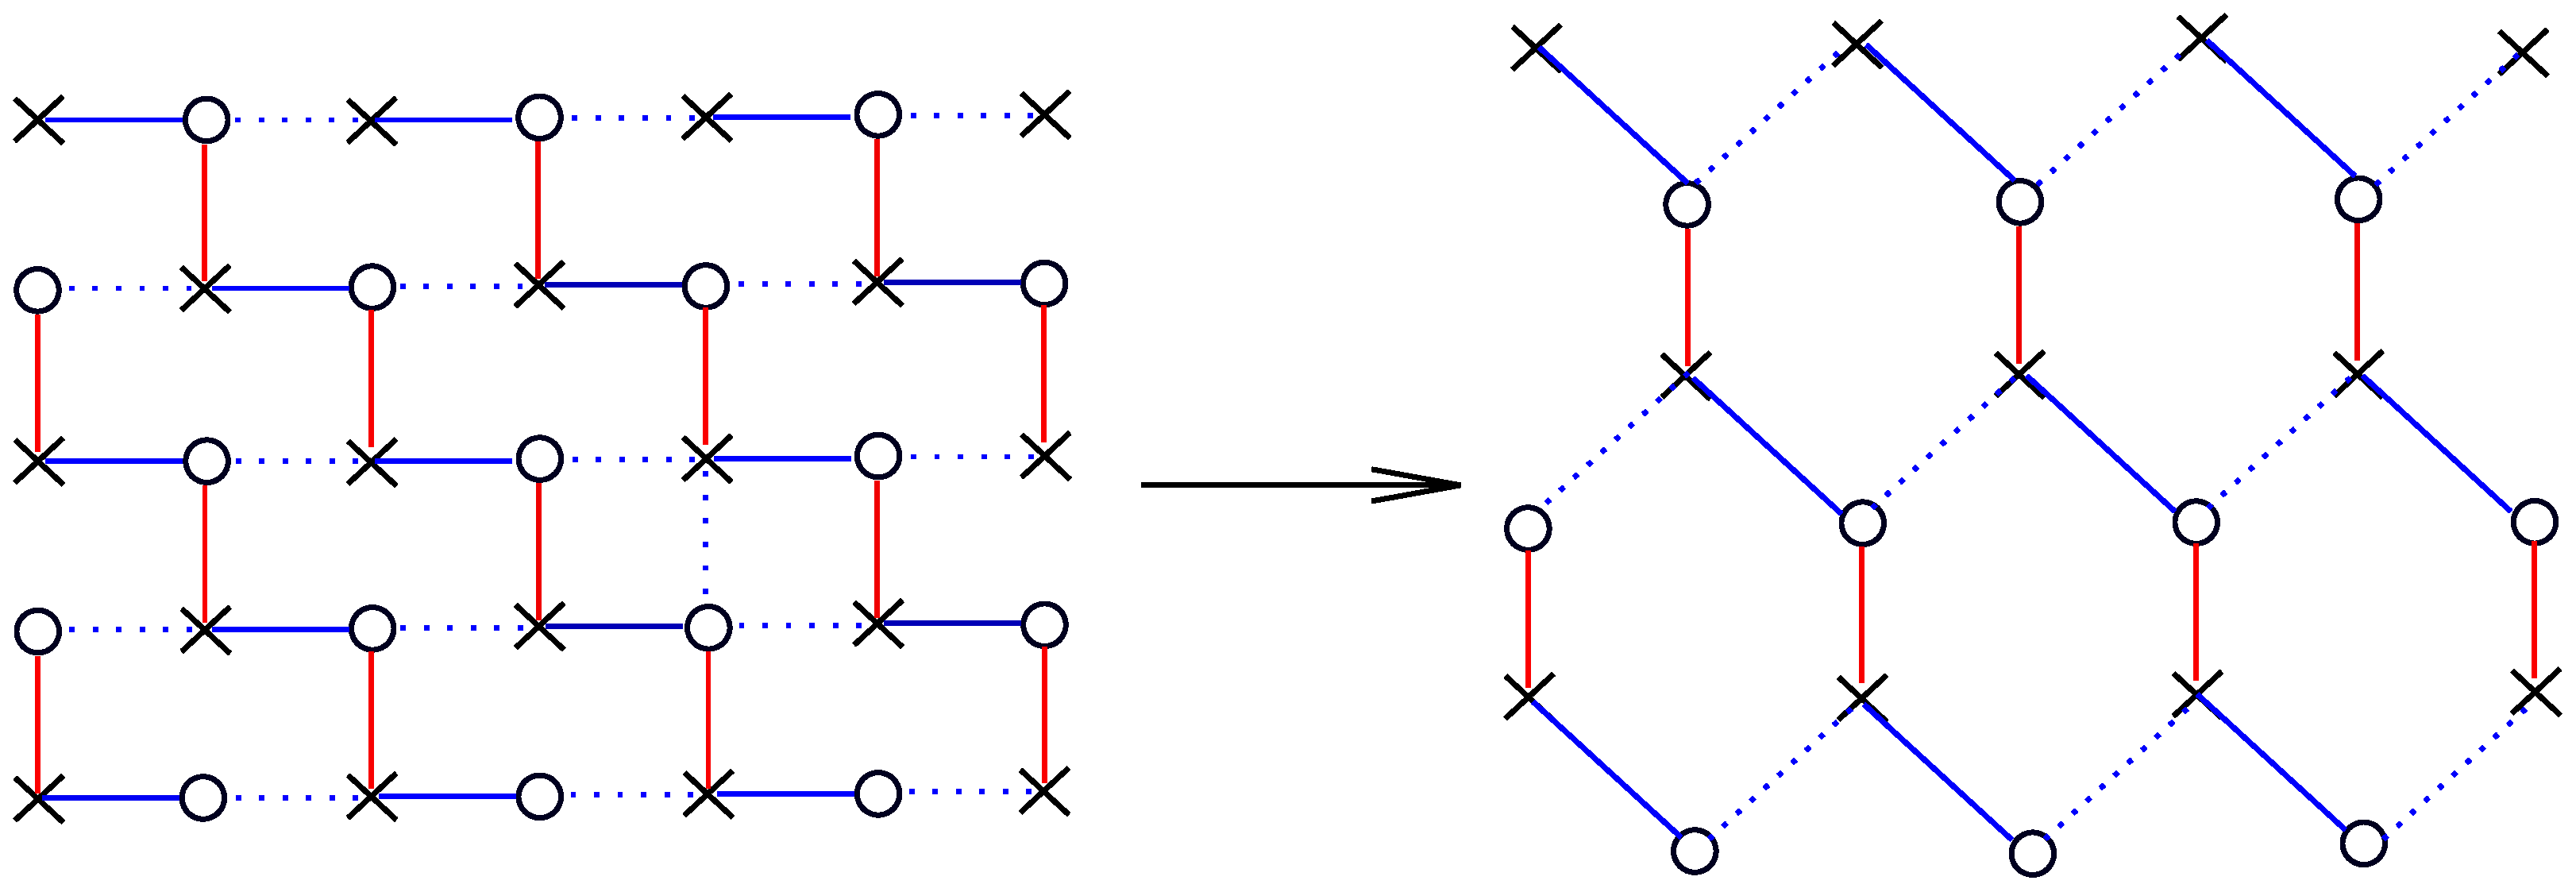
\includegraphics[width=1\linewidth]{part4/toHex.eps}}
	\caption{При $J_4 = 0$ обобщенная квадратная решетка превращается в так называемую кирпичную кладку, которая топологически эквивалентна гексагональной решетке}
	\label{hexTranf}
\end{figure}

При исследовании вариантов выбора знаков взаимодействий, установлено, что все они дают температурные зависимости энтропии и теплоемкости, представленные на рисунке~\ref{Hex}. И это не удивительно. Ведь, как известно~\cite{houtapell1950}, гексагональная решетка при любом выборе знаков взаимодействий не имеет фрустраций.

\begin{figure}[h]
	\begin{minipage}[h]{0.5\linewidth}
		\center{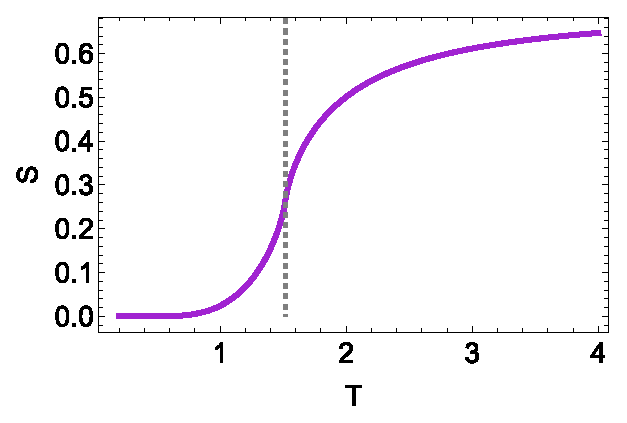
\includegraphics[width=1\linewidth]{part4/hexLatticeS.eps} \\ а)}
	\end{minipage}
	\hfill
	\begin{minipage}[h]{0.5\linewidth}
		\center{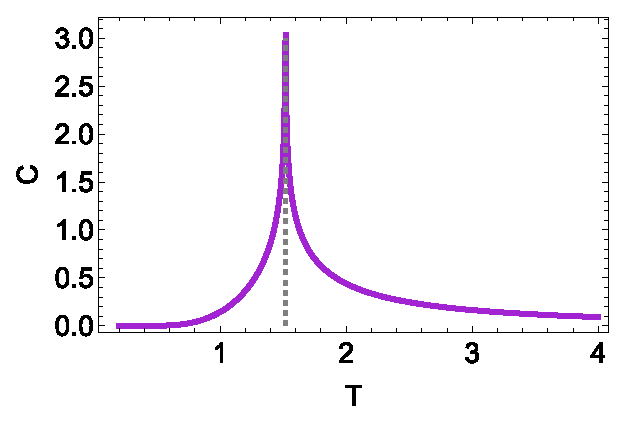
\includegraphics[width=1\linewidth]{part4/hexLatticeC.eps} \\ б)}
	\end{minipage}
	\caption{Температурные зависимости обобщенной квадратной решетки с тремя ненулевыми и одним нулевым взаимодействиями (гексагональная решетка): а) энтропия, б) теплоемкость. Пунктирной линией обозначена температура перехода гексагональной решетки: $T_c = 2/(\ln(2+\sqrt{3}))\approx 1.5187$.}
	\label{Hex}
\end{figure}

\begin{figure}[h]
	\begin{minipage}{0.45\linewidth}
		\center{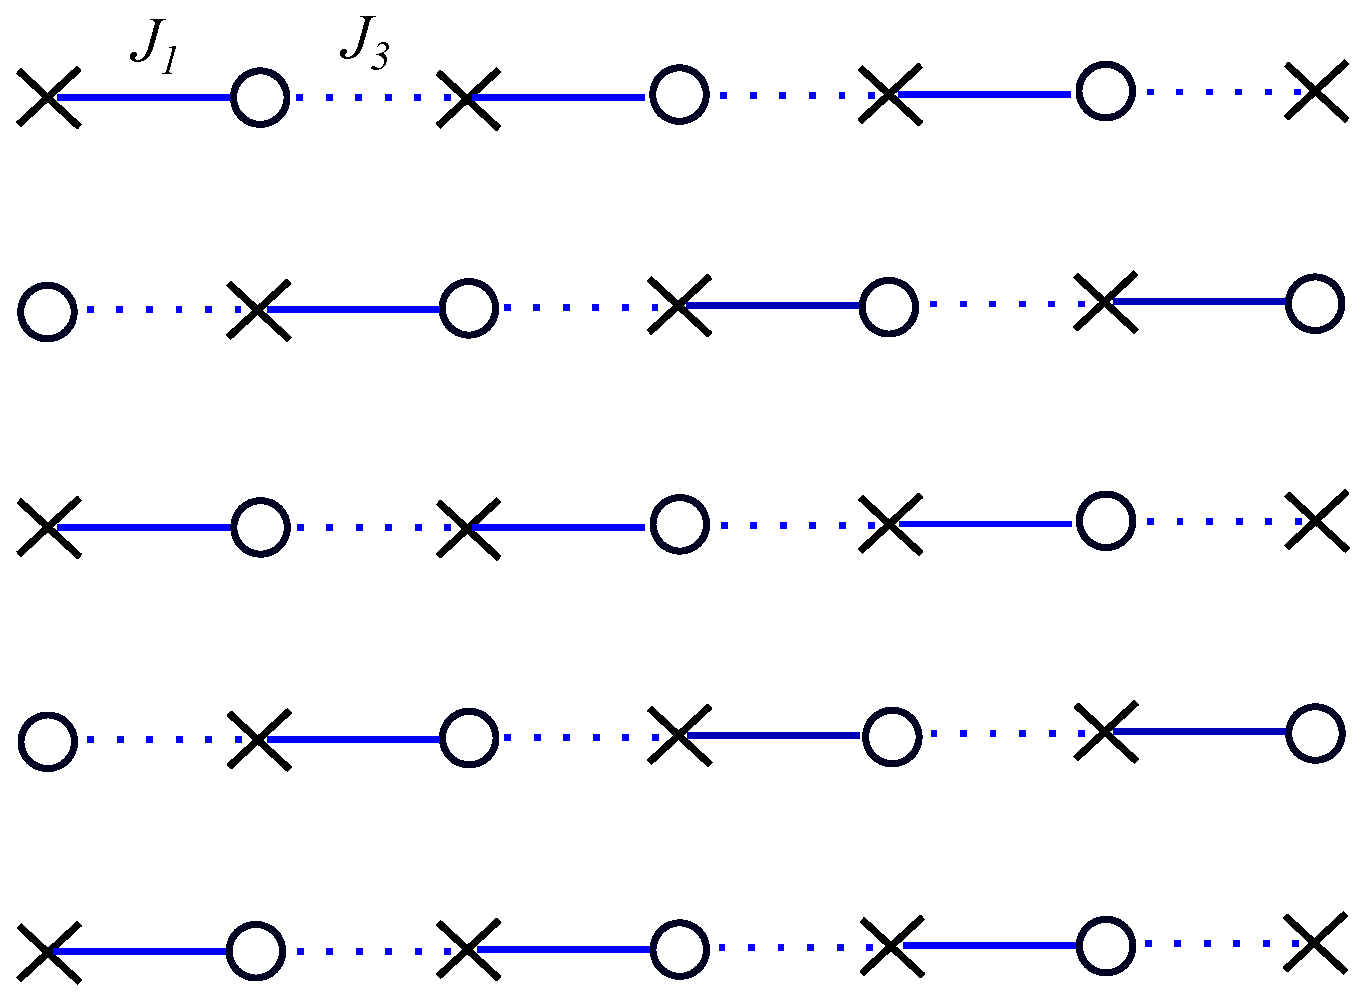
\includegraphics[width=1\linewidth]{part4/linear1.eps} \\ а)}
	\end{minipage}
	\hfill
	\begin{minipage}{0.45\linewidth}
		\center{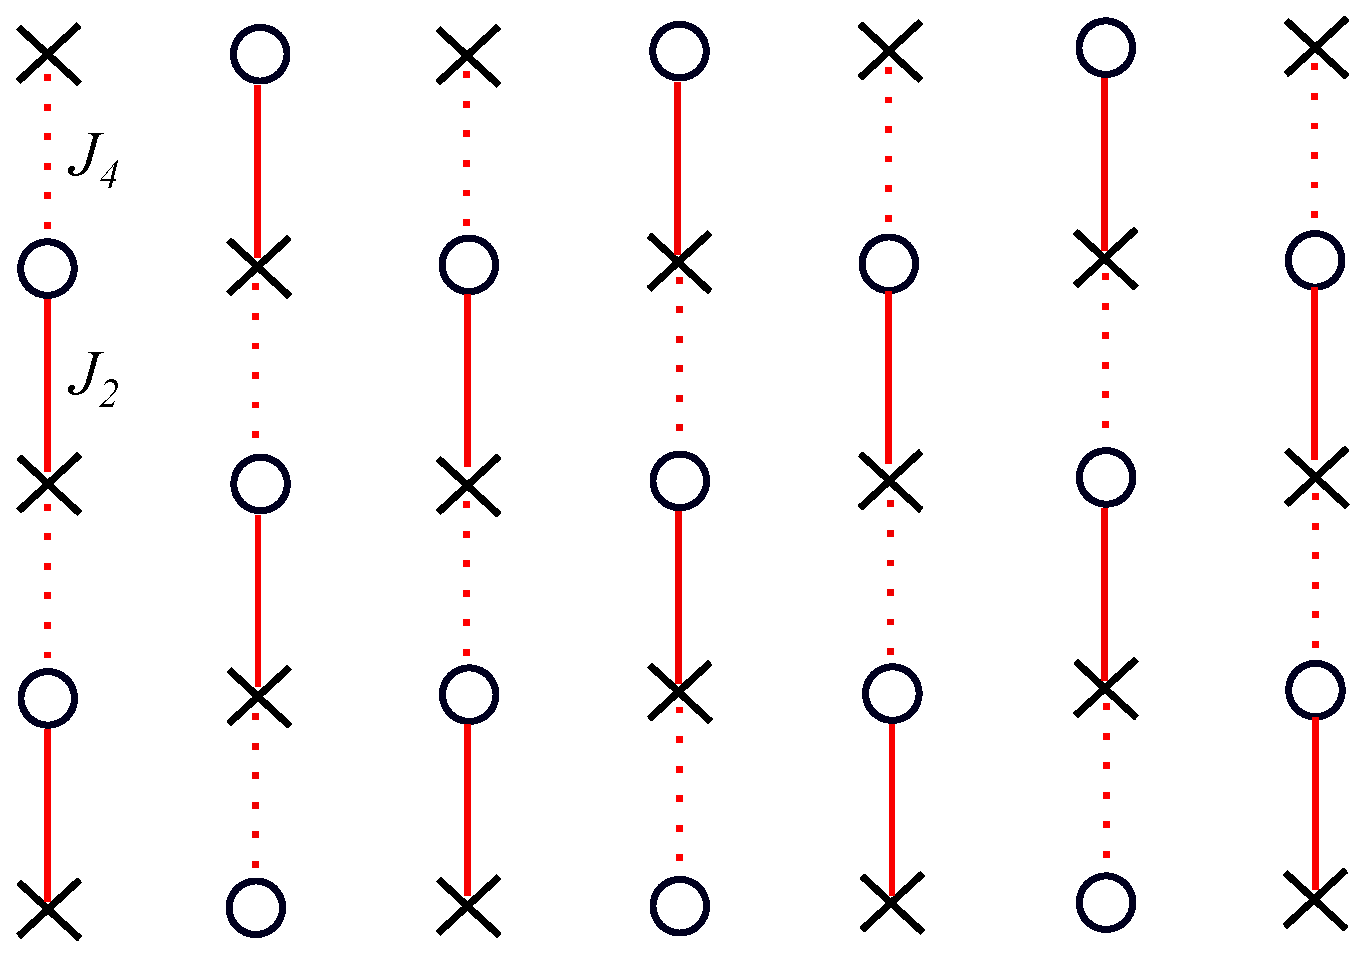
\includegraphics[width=1\linewidth]{part4/linear2.eps} \\ б)}
	\end{minipage}
	\vfill
	\begin{minipage}{0.45\linewidth}
		\center{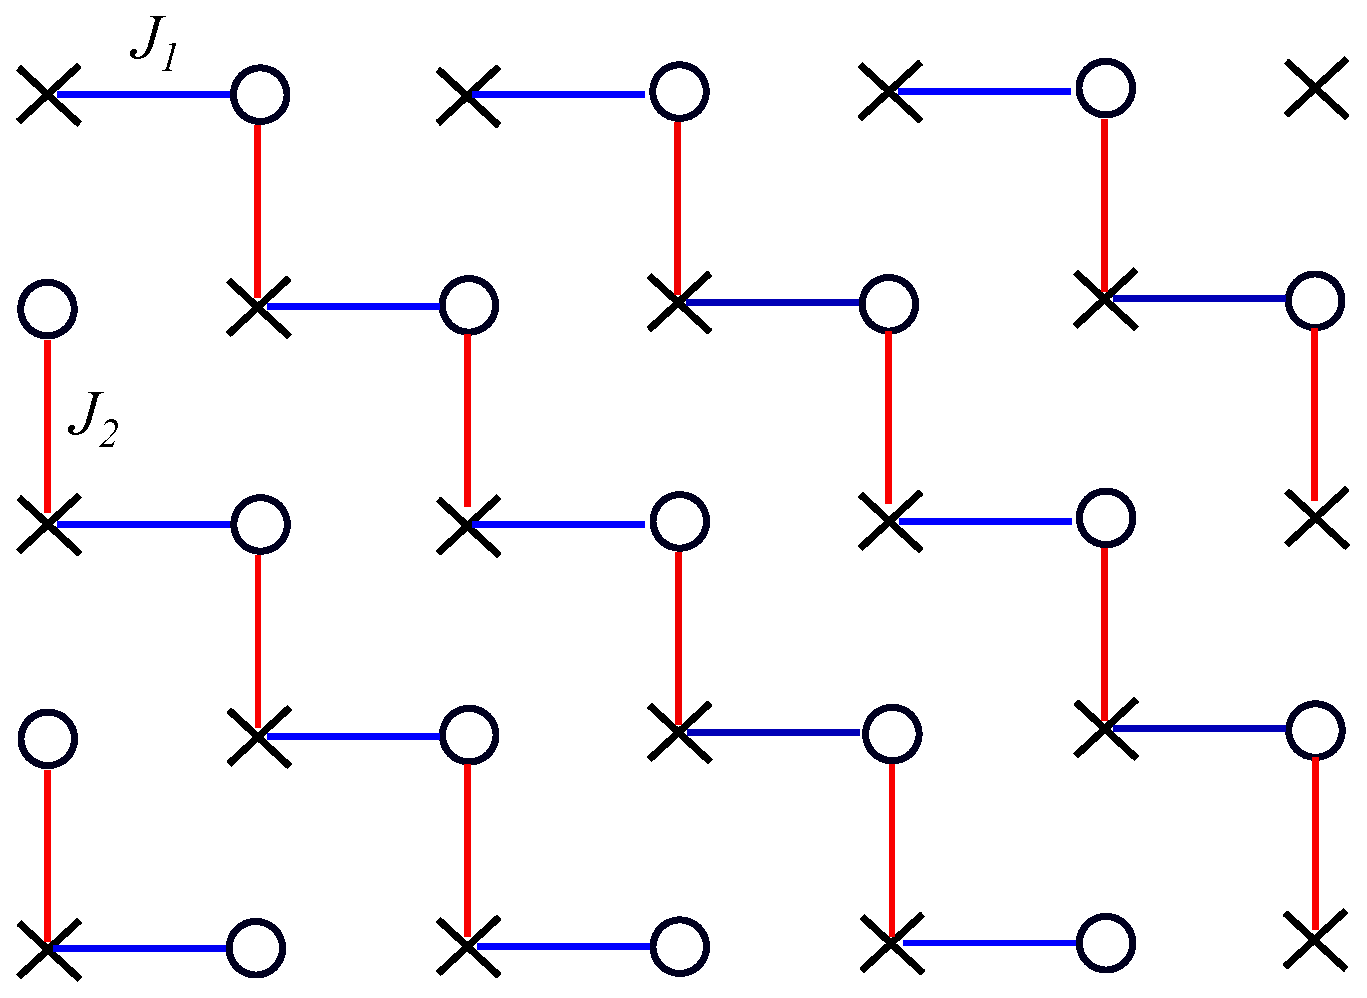
\includegraphics[width=1\linewidth]{part4/linear3.eps} \\ в)}
	\end{minipage}
	\hfill
	\begin{minipage}{0.45\linewidth}
		\center{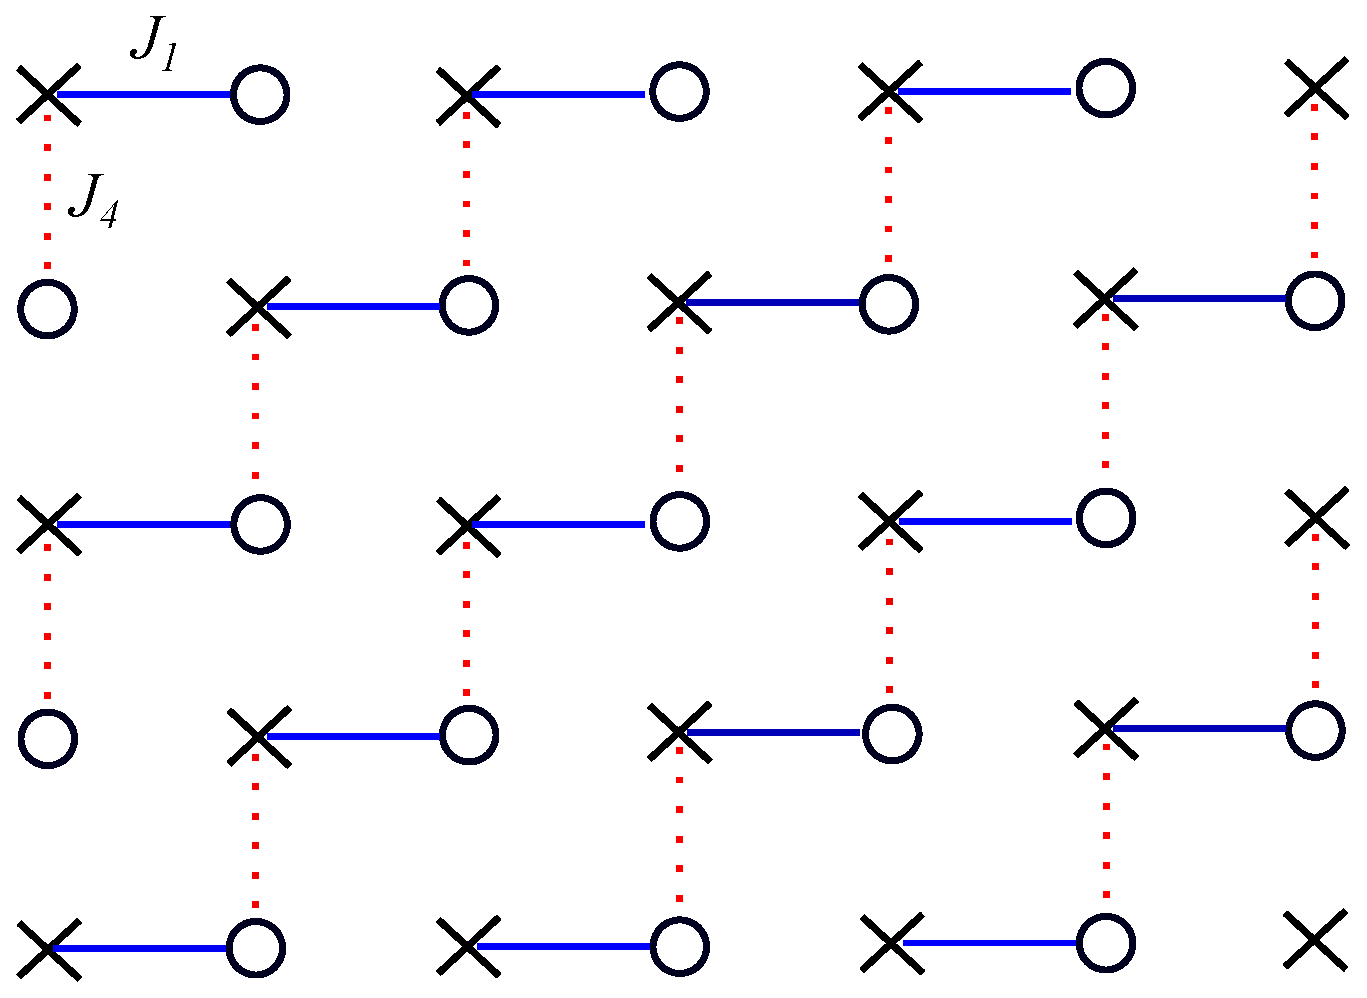
\includegraphics[width=1\linewidth]{part4/linear4.eps} \\ г)}	
	\end{minipage}
	\caption{а) и б) "Прямые" цепочки, в) и г) Цепочки "лестничного" типа.}
	\label{linearChains}
\end{figure}

Положив равным нулю сразу два обменных взаимодействия на обобщенной квадратной решетке получается линейная цепочка. Причем, эти цепочки можно получить разных видов. Так называемые "прямые" цепочки (рис.~\ref{linearChains}а и рис.~\ref{linearChains}б) и цепочки "лестничного" типа (рис.~\ref{linearChains}в и рис.~\ref{linearChains}г). Однако, все эти цепочки показывают одни и те же температурные зависимости энтропии и теплоемкости (рис.~\ref{Linear}). И, как известно~\cite{mussardo2010}, любая линейная цепочка не обнаруживает точки перехода, кроме $T=0$.

\begin{figure}[h]
	\begin{minipage}[h]{0.5\linewidth}
		\center{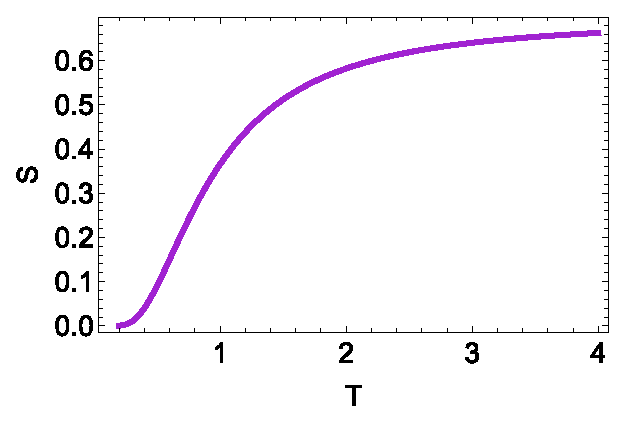
\includegraphics[width=1\linewidth]{part4/linearS.eps} \\ а)}
	\end{minipage}
	\hfill
	\begin{minipage}[h]{0.5\linewidth}
		\center{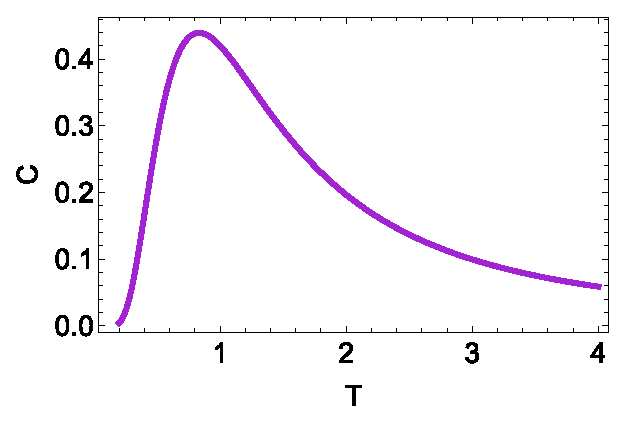
\includegraphics[width=1\linewidth]{part4/linearC.eps} \\ б)}
	\end{minipage}
	\caption{Температурные зависимости обобщенной квадратной решетки с двумя ненулевыми и двумя нулевыми взаимодействиями (линейная цепочка): а) энтропия, б) теплоемкость.}
	\label{Linear}
\end{figure}

Осталось рассмотреть случай зануления сразу трех взаимодействий из четырех, например, $J_2 = J_3 = J_4 = 0$. При таком выборе обменных взаимодействий получается решетка димеров, которая к тому же является фрустрированной. Нуль-температурная энтропия равна $\ln 2/2$.

\begin{figure}[h]
	\center{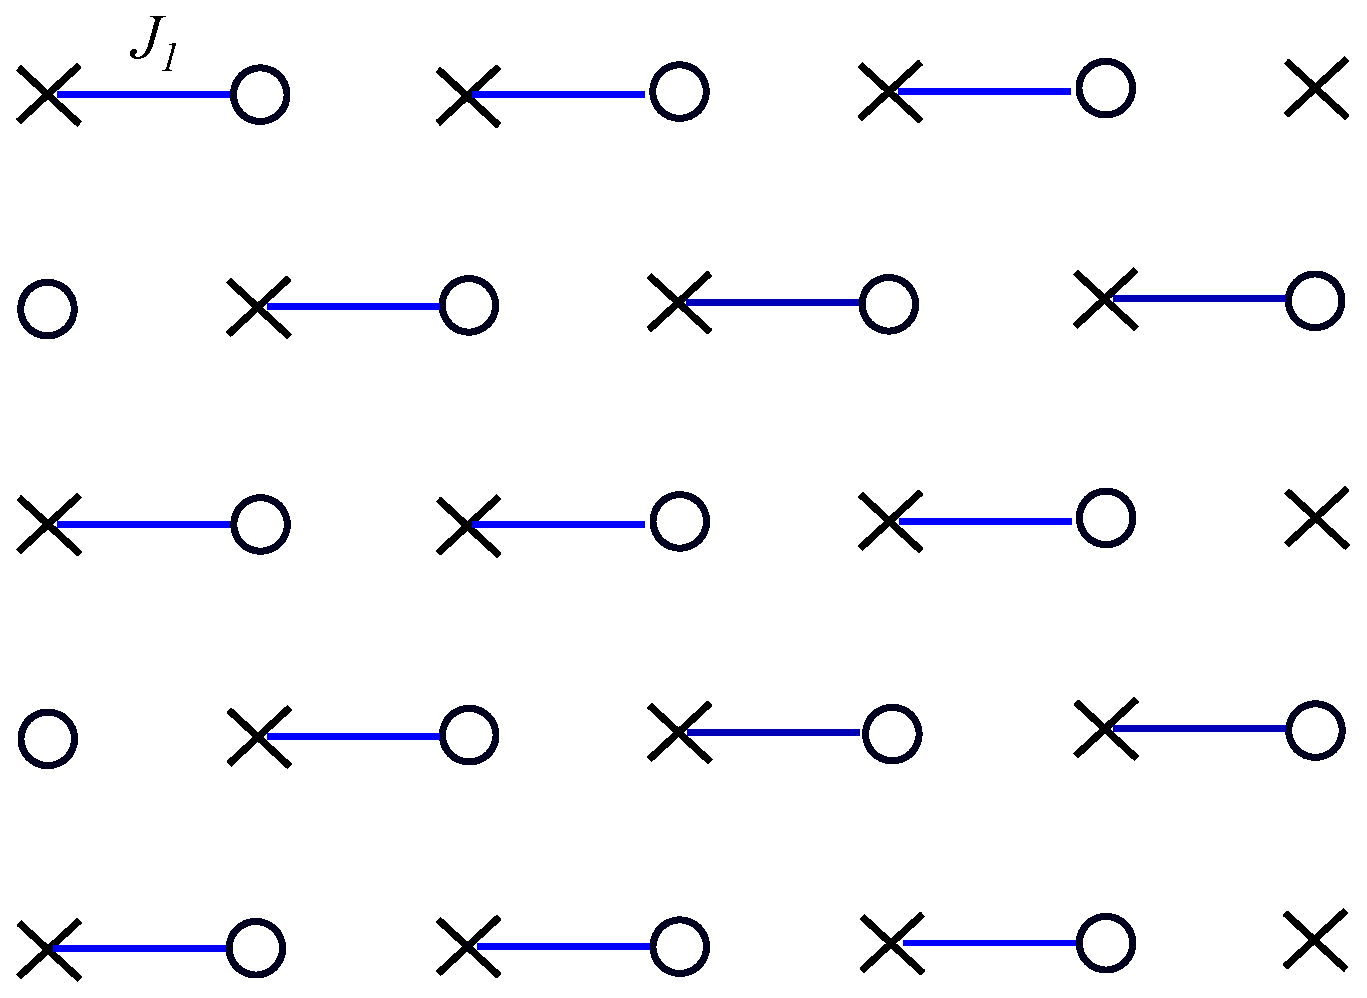
\includegraphics[width=0.45\linewidth]{part4/dimers.eps}}
	\caption{Решетка димеров, получаемая из обобщенной квадратной решетки, занулением любых трех взаимодействий, здесь $J_2 = J_3 = J_4 = 0$.}
	\label{dimerLattice}
\end{figure}

Взаимодействие между спинами в одном димере может быть либо ферромагнитным (спины параллельны), либо антиферромагнитным (спины антипараллельны). Таких пар, связанных спинов получается $N/2$, отсюда и двойка в знаменателе нуль-температурной энтропии. А так как пары спинов никак не влияют друг на друга, то направление спинов любой такой пары может не совпадать с направлением спинов соседних пар. Температурные зависимости энтропии и теплоемкости представлены на рисунке~\ref{Dimers}. Такие же зависимости получаются при занулении любых трех взаимодействий на обобщенной квадратной решетке вне зависимости от знака оставшегося взаимодействия (антиферромагнитное или ферромагнитное).

\begin{figure}[h]
	\begin{minipage}[h]{0.5\linewidth}
		\center{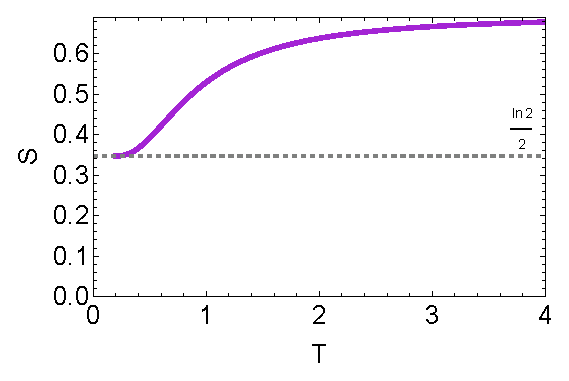
\includegraphics[width=1\linewidth]{part4/dimersS.eps} \\ а)}
	\end{minipage}
	\hfill
	\begin{minipage}[h]{0.5\linewidth}
		\center{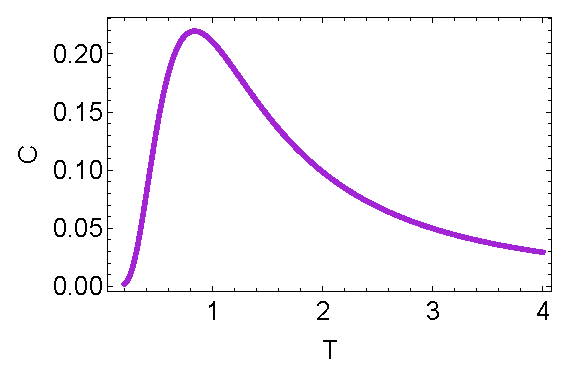
\includegraphics[width=1\linewidth]{part4/dimersC.eps} \\ б)}
	\end{minipage}
	\caption{Температурные зависимости обобщенной квадратной решетки с тремя нулевыми и одним ненулевым взаимодействиями (решетка димеров): а) энтропия, б) теплоемкость. Пунктирной линией обозначена нуль-температурная энтропия: $S_{T\rightarrow 0} = \ln 2/2\approx 0.34657$.}
	\label{Dimers}
\end{figure}

Наконец, когда сразу все взаимодействия равны нулю $J_1 = J_2 = J_3 = J_4 = 0$, получается, что энтропия вне зависимости от температуры всегда будет равна одну и тому же значению, $\ln 2$. Поскольку изначально рассматривается энтропия на один узел решетки $S/N$, этот результат неудивителен и означает, что каждый спин в решетке может принимать два значения (спин вверх или спин вниз). Так как в решетке уже нет взаимодействия между спинами, то спины свободны и могут ориентироваться случайно. Это состояние в системе называется парамагнитным. Именно это состояние системы получается, когда температура устремляется к бесконечности. 

Вернемся к рассмотрению четырех ненулевых обменных взаимодействий на обобщенной квадратной решетке, а именно к случаю $J_1 = -1, J_2 = -1, J_3 = -1, J_4 = 1$ (или $J_1 = 1, J_2 = 1, J_3 = 1, J_4 = -1$). Уже известно, что при таком выборе параметров обменного взаимодействия решетка будет фрустрированной с нуль-температурной энтропией равной $G/\pi$ (рис.~\ref{Catalan}). 

Начнем увеличивать ферромагнитное значение $J_4$, а остальные взаимодействия останутся прежними. Температурные зависимости энтропий для некоторых значений обменных взаимодействий проиллюстрированы на рисунке~\ref{Peak}. При этом видно, что приведенные температурные зависимости энтропий, для которых $J_4>1$, имеют одно общее значение при $T \rightarrow 0$. 

\begin{figure}[h]
	\begin{minipage}[h]{0.5\linewidth}
		\center{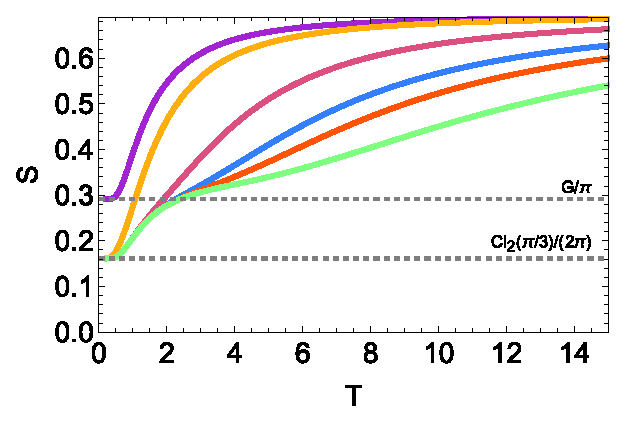
\includegraphics[width=1\linewidth]{part4/peakS.eps} \\ а)}
	\end{minipage}
	\hfill
	\begin{minipage}[h]{0.5\linewidth}
		\center{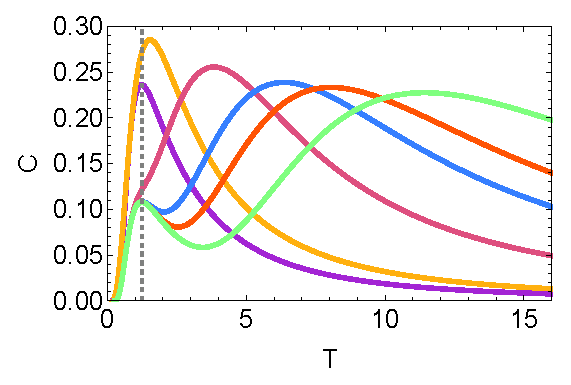
\includegraphics[width=1\linewidth]{part4/peakC.eps} \\ б)}
	\end{minipage}
	\caption{Температурные зависимости обобщенной квадратной решетки для различных параметров обменных взаимодействий: фиолетовая кривая --- $J_1 = -1$, $J_2 = -1$, $J_3 = -1$, $J_4 = 1$, желтая кривая --- $J_1 = -1$, $J_2 = -1$ , $J_3 = -1$, $J_4 = 2$, розовая кривая --- $J_1 = -1$, $J_2 = -1$ , $J_3 = -1$, $J_4 = 5$, синяя кривая --- $J_1 = -1$, $J_2 = -1$, $J_3 = -1$, $J_4 = 8$, красная кривая --- $J_1 = -1$, $J_2 = -1$ , $J_3 = -1$, $J_4 = 10$, зеленая кривая --- $J_1 = -1$, $J_2 = -1$ , $J_3 = -1$, $J_4 = 14$: а) энтропия. Пунктирными линиями обозначены значения нуль-температурных энтропий: $S_{T\rightarrow 0} = G/\pi\approx 0.29156$, где $G$ --- постоянная Каталана, $S_{T\rightarrow 0} = \frac{1}{2\pi} \Cl_2 (\frac{\pi}{3})\approx0.16153$, где $\Cl_2 (\varphi)$ --- функция Клаузена. б) теплоемкость. Пунктирной линией обозначено положение малого гладкого пика ($T_{peak}\approx1.232$). }
	\label{Peak}
\end{figure}

Установлено, что нуль-температурное значение для энтропий, когда $J_4>1$, выражается в виде    
\begin{equation}
	S_{T\rightarrow 0} = \frac{1}{2\pi} \Cl_2 \bigg(\frac{\pi}{3}\bigg)   = 0.16153\dots, 
	\label{cl}
\end{equation} 
где  $\Cl_2 (\varphi)$ --- функция Клаузена. Функция Клаузена --- трансцендентная специальная функция одной переменной, которая связана с мнимой частью дилогарифма $\Li_2$
\begin{equation*}
	\Cl_2 (\varphi) = \im (\Li_2 (e^{i \varphi})).
\end{equation*}

Кроме того, функция Клаузена может быть записана через различные интегральные представления, которые можно найти в математическом справочниках и статьях (например, \cite{abramowitz_stegun1972, wood1968}).

Интересно то, что постоянную Каталана так же можно выразить через функцию Клаузена~\cite{wood1968}
\begin{equation*}
	G = \Cl_2 \bigg(\frac{\pi}{2}\bigg) = \im (\Li_2 (i)),
\end{equation*}

\noindent поэтому фрустрационное значение энтропии в выражении \eqref{g} может быть переписано в виде
\begin{equation}
	\frac{G}{\pi} = \frac{1}{\pi} \Cl_2 \bigg(\frac{\pi}{2}\bigg) = 0.29156\dots
\end{equation}

Кроме того, при увеличение ферромагнитного значения $J_4$ можно заметить нехарактерную особенность, связанную с теплоемкостью~(рис.~\ref{Peak}). Начиная со значения $J_4 = 5$ (розовая кривая на рисунке~\ref{Peak}б), формируется дополнительный гладкий пик теплоемкости, в то время как большой гладкий пик растягивается и смещается вправо. Более того положение дополнительного гладкого пика теплоемкости не меняется относительно увеличения ферромагнитного значения $J_4$, в то время как большой пик теплоемкости постоянно меняется. Что же касается энтропий, то их нуль-температурные значения при $J_4>1$ равны одному и тому же значению $\frac{1}{2\pi} \Cl_2 (\frac{\pi}{3})$. Все те же рассуждения справедливы для случая, когда $J_1 = 1, J_2 = 1, J_3 = 1$ и антиферромагнитном увеличении $J_4$.

Такое поведение необычно для фрустрированной системы, поэтому это требует дополнительного исследования.  

\begin{figure}[h]
	\begin{minipage}[h]{0.5\linewidth}
		\center{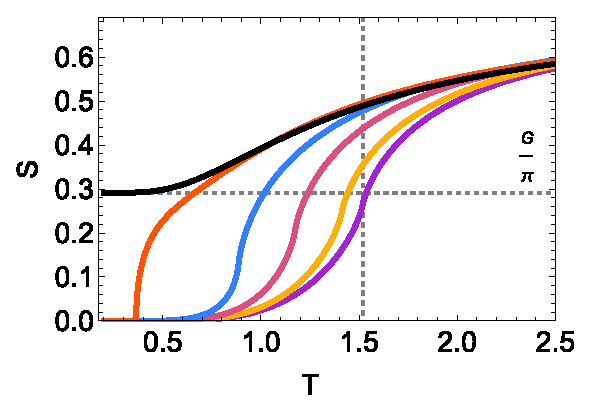
\includegraphics[width=1\linewidth]{part4/peak2S.eps} \\ а)}
	\end{minipage}
	\hfill
	\begin{minipage}[h]{0.5\linewidth}
		\center{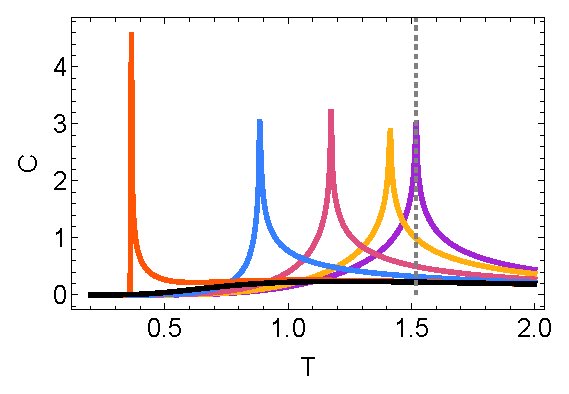
\includegraphics[width=1\linewidth]{part4/peak2C.eps} \\ б)}
	\end{minipage}
	\caption{Температурные зависимости обобщенной квадратной решетки для различных параметров обменных взаимодействий: фиолетовая кривая --- $J_1 = -1$, $J_2 = -1$, $J_3 = -1$, $J_4 = 0$, желтая кривая --- $J_1 = -1$, $J_2 = -1$ , $J_3 = -1$, $J_4 = 0.1$, розовая кривая --- $J_1 = -1$, $J_2 = -1$ , $J_3 = -1$, $J_4 = 0.3$, синяя кривая --- $J_1 = -1$, $J_2 = -1$, $J_3 = -1$, $J_4 = 0.5$, красная кривая --- $J_1 = -1$, $J_2 = -1$ , $J_3 = -1$, $J_4 = 0.8$, черная кривая --- $J_1 = -1$, $J_2 = -1$ , $J_3 = -1$, $J_4 = 1$: а) энтропия. Пунктирными линиями обозначены значение нуль-температурной энтропии: $S_{T\rightarrow 0} = G/\pi\approx 0.29156$, где $G$ --- постоянная Каталана и значение точки перехода для гексагональной решетки $T_c = 2/(\ln(2+\sqrt{3}))\approx 1.5187$. б) теплоемкость. Пунктирной линией обозначено значение точки перехода для гексагональной решетки $T_c = 2/(\ln(2+\sqrt{3}))\approx 1.5187$. }
	\label{Peak2}
\end{figure}

Рассмотрим поведение системы при приближении к точке фрустрации с обменными взаимодействиями $J_1 = -1$, $J_2 = -1$, $J_3 = -1$, $J_4 = 1$ (черная кривая на рисунке~\ref{Peak2}). Начнем с параметров $J_1 = -1$, $J_2 = -1$, $J_3 = -1$, $J_4 = 0$. Мы уже знаем, что при таком выборе взаимодействий реализуется случай гексагональной решетки~(рис.~\ref{Hex}). Энтропия и теплоемкость гексагональной решетки изображены фиолетовой кривой на рисунках \ref{Peak2}а и \ref{Peak2}б соответственно. Будем постепенно увеличивать ферромагнитное значение параметра $J_4$ от $0$ до $1$. Глядя на рисунки \ref{Peak2}а и \ref{Peak2}б, можно сделать сразу несколько выводов. Во-первых, зависимости теплоемкостей изображены в виде $\Lambda$ -- образных пиков. Это значит, что в точках, где теплоемкость испытывает скачок, имеет место фазовый переход. Следовательно, в этих точках не наблюдается бесконечного числа конфигураций с одинаковой энергией, иначе говоря, фрустрации отсутствуют. Во-вторых, при приближении к точке фрустрации $J_1 = -1$, $J_2 = -1$, $J_3 = -1$, $J_4 = 1$ (черная кривая на рисунке~\ref{Peak2}) зависимости теплоемкостей, смещаясь влево по температуре, испытывают укручение левой части графика.

\begin{figure}[h]
	\begin{minipage}[h]{0.5\linewidth}
		\center{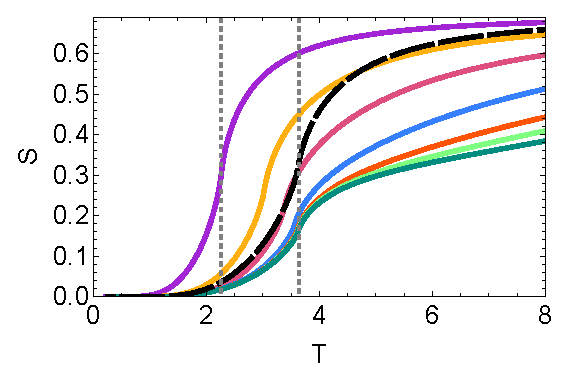
\includegraphics[width=1\linewidth]{part4/triangularS.eps} \\ а)}
	\end{minipage}
	\hfill
	\begin{minipage}[h]{0.5\linewidth}
		\center{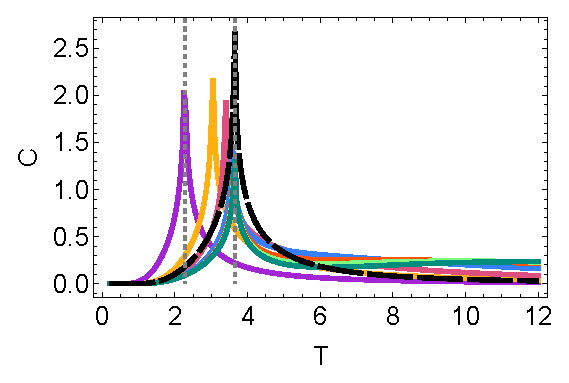
\includegraphics[width=1\linewidth]{part4/triangularC.eps} \\ б)}
	\end{minipage}
	\caption{Температурные зависимости обобщенной квадратной решетки для различных параметров обменных взаимодействий: фиолетовая кривая --- $J_1 = 1$, $J_2 = 1$, $J_3 = 1$, $J_4 = 1$, желтая кривая --- $J_1 = 1$, $J_2 = 1$ , $J_3 = 1$, $J_4 = 3$, розовая кривая --- $J_1 = 1$, $J_2 = 1$ , $J_3 = 1$, $J_4 = 5$, синяя кривая --- $J_1 = 1$, $J_2 = 1$, $J_3 = 1$, $J_4 = 8$, красная кривая --- $J_1 = 1$, $J_2 = 1$ , $J_3 = 1$, $J_4 = 11$, зеленая кривая --- $J_1 = 1$, $J_2 = 1$ , $J_3 = 1$, $J_4 = 13$, темно-зеленая кривая --- $J_1 = 1$, $J_2 = 1$ , $J_3 = 1$, $J_4 = 15$: а) энтропия, б) теплоемкость. Серыми пунктирными линиями обозначены значения точек перехода для квадратной и треугольной решеток соответственно: $T_c = 2/(\ln(1+\sqrt{2}))\approx 2.2692$,  $T_c = 4/\ln 3\approx 3.64096$. Черной пунктирной линией обозначены температурные зависимости энтропии и теплоемкости треугольной решетки с параметрами $J_1 = J_2 = J_3 = 1$.}
	\label{Triangular}
\end{figure}

\begin{figure}[h]
	\center{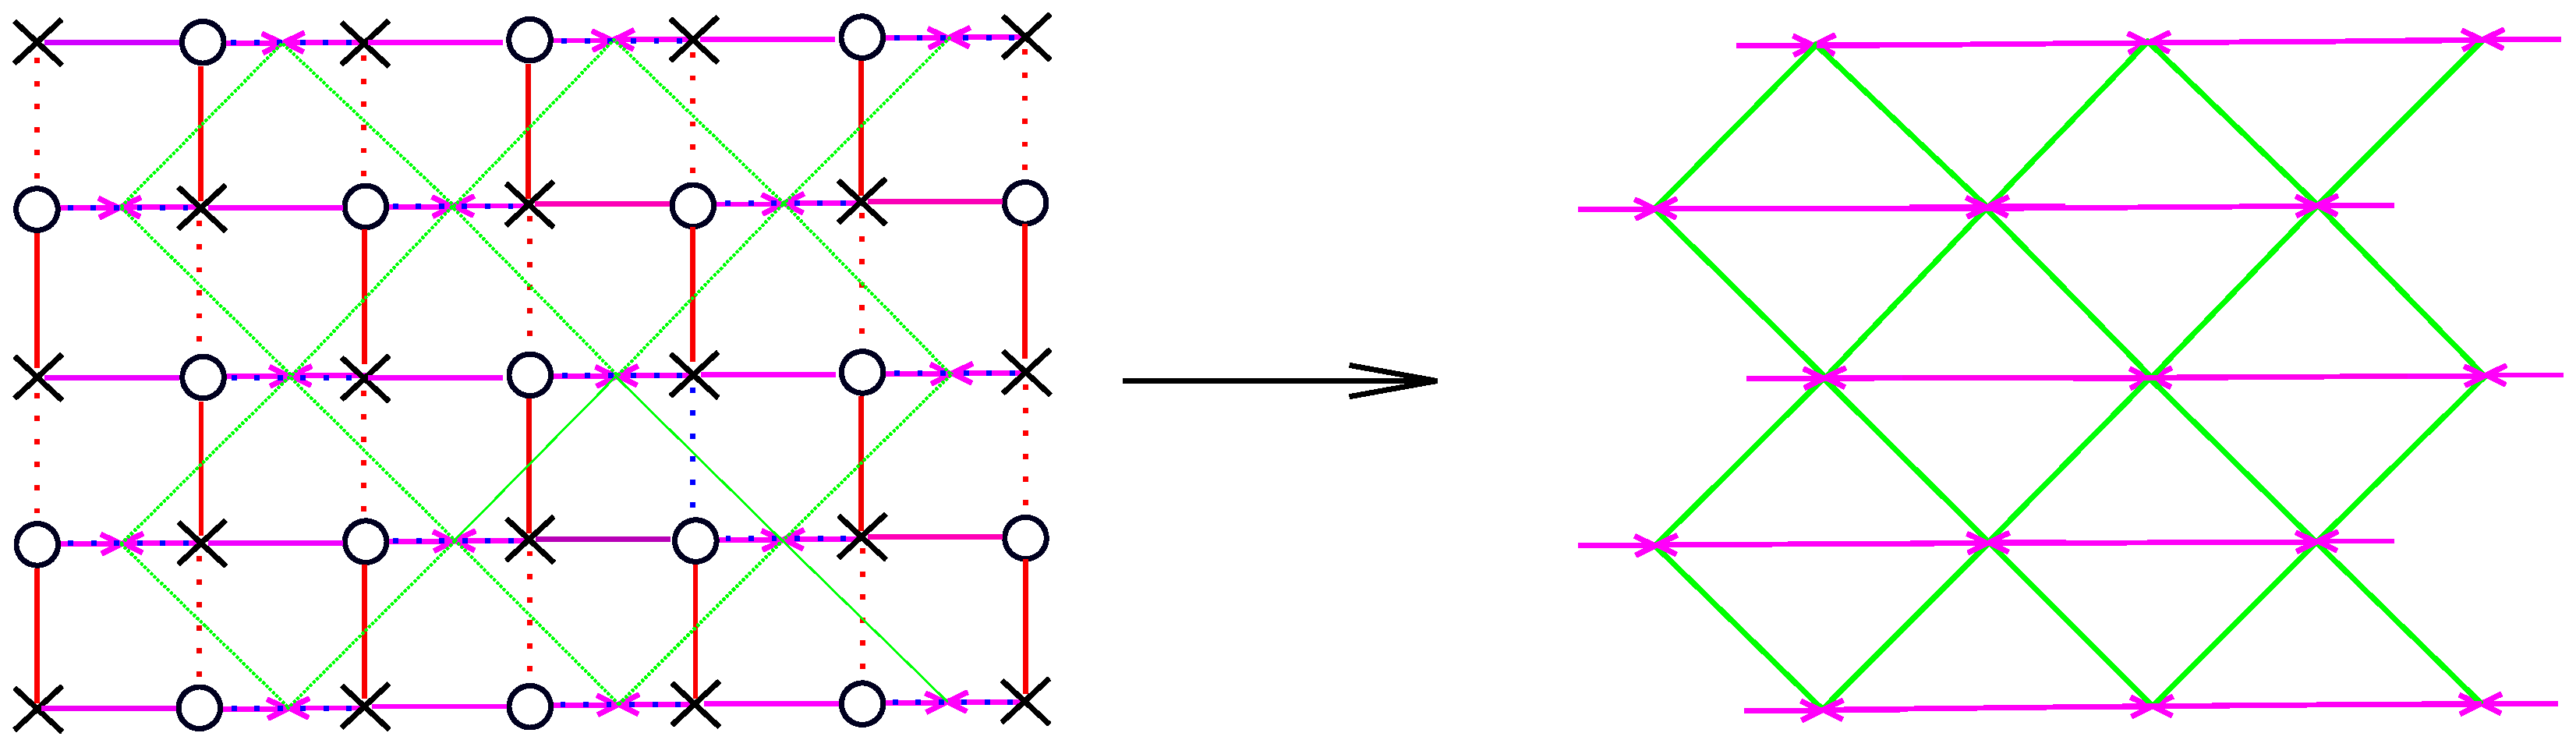
\includegraphics[width=1\linewidth]{part4/toTriag.eps}}
	\caption{Преобразование обобщенной квадратной решетки к треугольной решетке, устремляя одно из обменных взаимодействий к бесконечности}
	\label{triag}
\end{figure}

До сих пор мы не рассмотрели еще один частный случай, о котором уже ранее говорили~\cite{confbib6}. Пусть параметры обменного взаимодействия равны $J_1 = J_2 = J_3 = J_4 = 1$ (фиолетовая кривая на рисунке~\ref{Triangular}). Этот случай уже известен и реализует обычную онзагеровскую квадратную решетку с температурой перехода $T_c = \frac{2}{\ln (1+\sqrt{2})}$~\cite{kramers_wannier1, kramers_wannier2}. При увеличении ферромагнитного взаимодействия $J_4$, энтропии и теплоемкости сходятся к некоторой точке перехода. Подтверждением этого факта служат рисунки \ref{Triangular}а и \ref{Triangular}б. Это ни что иное как температура перехода для треугольной решетки, $T_c = \frac{4}{\ln 3}$~\cite{wannier1950}. Треугольную решетку в данном случае можно получить, устремив любое из взаимодействий в бесконечность. Таким образом, обобщенная квадратная решетка сводится к треугольной решетке. Подтверждением этого является рисунок~\ref{triag}. 

Когда мы рассматривали обобщенную квадратную решетку с параметрами $J_1 = -1, J_2 =-1, J_3 = -1$ и $J_4 > 0$, происходило все то же самое. Обобщенная квадратная решетка превращалась в другую решетку под действием увеличения взаимодействия $J_4$. Но на самом деле увеличить $J_4$ мы можем только до какого-то конечного числа, а не до бесконечности. Поэтому получаем мы не треугольную решетку, а топологически искаженную решетку Кагоме~(рис.~\ref{kagomelike}). Такая решетка содержит шестиугольники и треугольники разных размеров (в отличие от обычной решетки Кагоме, в которой треугольники одного размера). 

\begin{figure}[h]
	\center{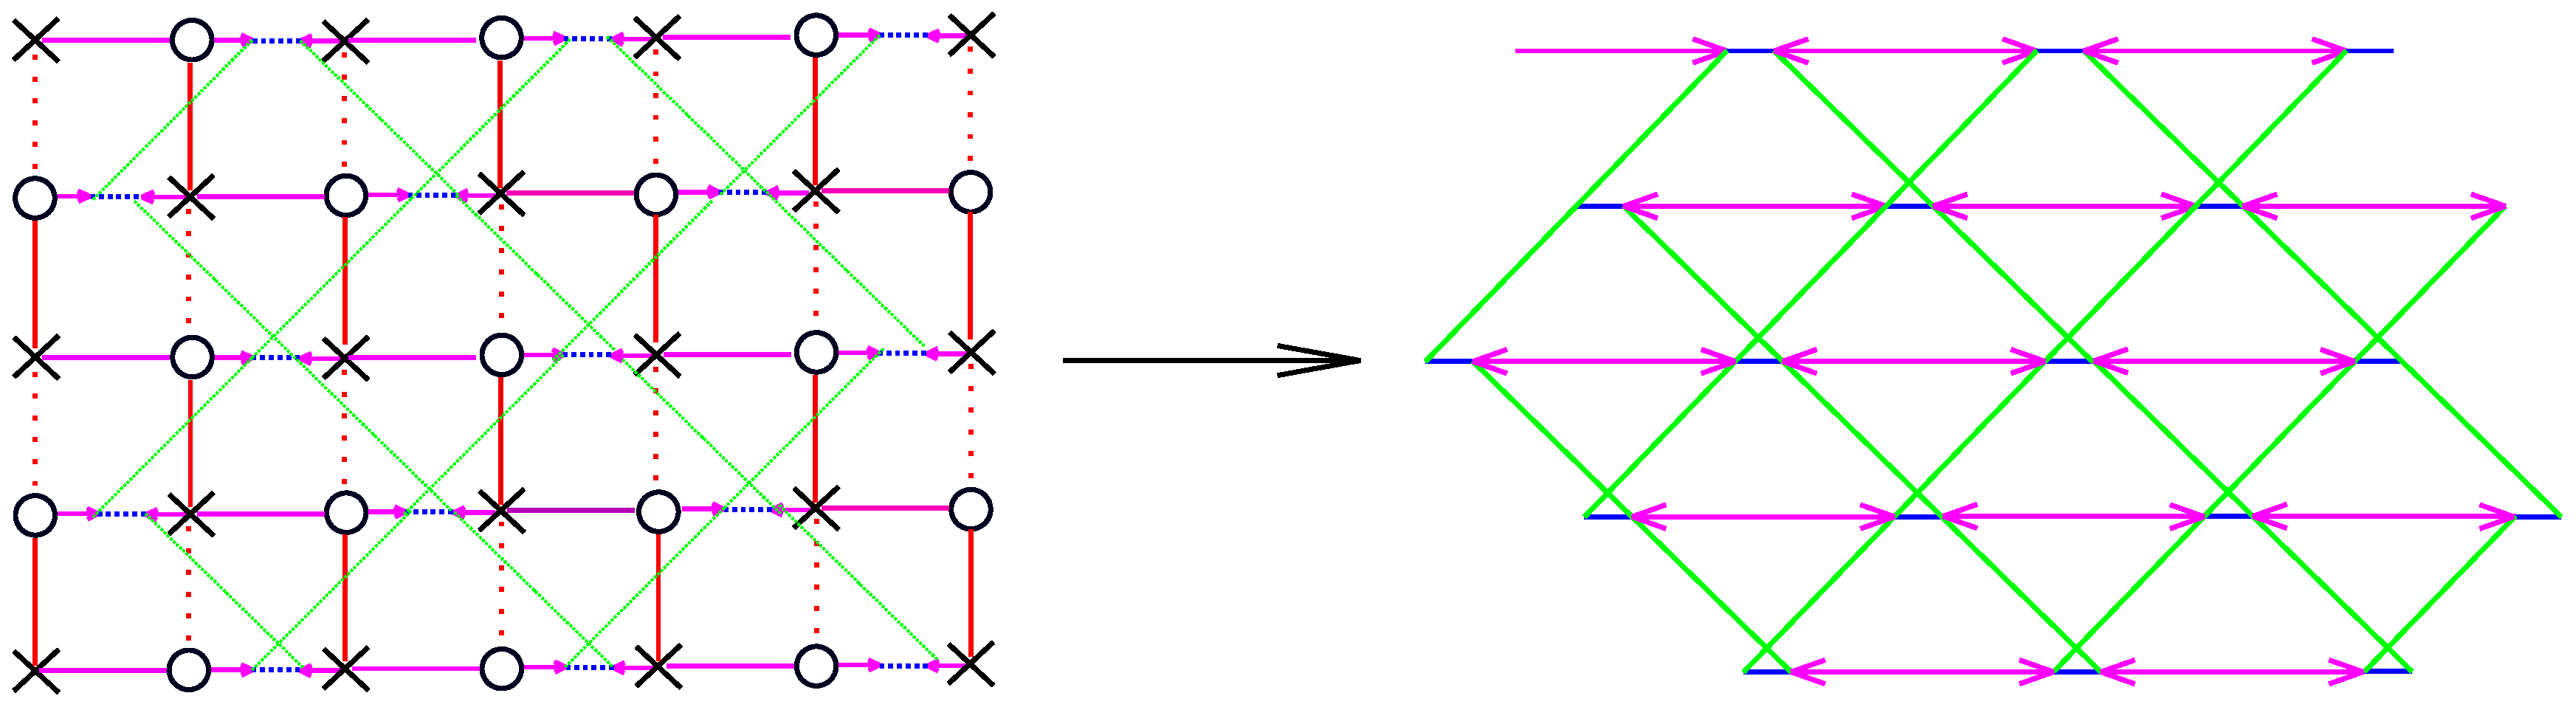
\includegraphics[width=1\linewidth]{part4/kagomelike.eps}}
	\caption{Получение кагоме подобной решетки из обобщенной модели Изинга при конечном увеличении одного из параметров обменного взаимодействия}
	\label{kagomelike}
\end{figure}

Напомним, что на данной решетке мы получили фрустрацию при $J_1 = -1, J_2 =-1, J_3 = -1, J_4 = 1$, а также при дальнейшем увеличении $J_4$ состояние мало того, что остается фрустрированным, так еще и все значения нуль-температурной энтропии равны одному и тому же значению $\frac{1}{2\pi} \Cl_2 (\frac{\pi}{3})$, а теплоемкость имеет дополнительный гладкий пик.

\section{Частные случаи обобщенной модели Изинга на квадратной решетке}

\subsection{Обычная квадратная решетка}
 
Если положить, что $J_1 = J_3$ и $J_2 = J_4$, то обобщенная модель Изинга на квадратной решетке сводится к обычной модели Изинга на квадратной решетке. Решение обычной модели Изинга было подробно исследовано в Главе~\ref{ch:ch1}. Также, мы увидели, что квадратная решетка при любых параметрах обменного взаимодействия в отсутствие магнитного поля не является фрустрированной.

 \begin{figure}[h]
     \center{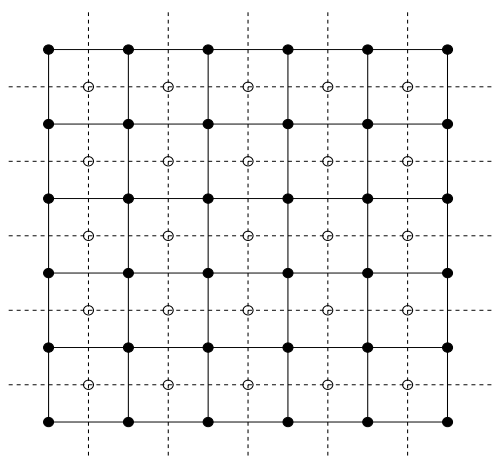
\includegraphics[width=0.5\linewidth]{part4/dualSquare.png}}
     \caption{Самодуальность квадратной решетки~\cite{mussardo2010}}
     \label{dualSquare}
 \end{figure}

Кроме того, квадратная решетка является самодуальной, то есть она дуальна сама себе~(рисунок~\ref{dualSquare}). Температура перехода --- $T_c^{square} = J\cdot 2.2692\dots$.

\subsection{Треугольная решетка} 

Переход от обобщенной квадратной решетки к треугольной осуществляется при стремлении одного взаимодействия к бесконечности. На рисунке \ref{toTriag} мы устремляли к бесконечности обменное взаимодействие $J_1$.  

Точное решение для треугольной решетки можно получить комбинаторным методом Вдовиченко--Фейнмана. 
Матрица коэффициентов $\Lambda$ треугольной решетки может быть записана в виде
\begin{multline}
\Lambda (p, q, \mu\; |\; p, q, \mu^{'}) = \\ =
\begin{pmatrix}
y \epsilon^{-p} & x \alpha^{-1} \epsilon^{-p-q}  &  z \alpha^{-2} \epsilon^{-q}  &  0  &  x \alpha^2 \epsilon^{p+q}  &  z \alpha \epsilon^{q} \\
y \alpha \epsilon^{-p} & x \epsilon^{-p-q}  &  z \alpha^{-1} \epsilon^{-q}  &  y \alpha^{-2} \epsilon^{p}  &  0  &  z \alpha^2 \epsilon^{q} \\
y \alpha^2 \epsilon^{-p} & x \alpha \epsilon^{-p-q}  &  z \epsilon^{-q}  &  y \alpha^{-1} \epsilon^{p}  &  x \alpha^{-2} \epsilon^{p+q}  &  0 \\
0 & x \alpha^{2} \epsilon^{-p-q}  &  z \alpha \epsilon^{-q}  &  y \epsilon^{p}  &  x \alpha^{-1} \epsilon^{p+q}  &  z \alpha^{-2} \epsilon^{q} \\
y \alpha^{-2} \epsilon^{-p} & 0  &  z \alpha^{2} \epsilon^{-q}  &  y \alpha \epsilon^{p}  &  x \epsilon^{p+q}  &  z \alpha^{-1} \epsilon^{q} \\
y \alpha^{-1} \epsilon^{-p} & x \alpha^{-2} \epsilon^{-p-q}  &  0  &  y \alpha^{2} \epsilon^{p}  &  x \alpha \epsilon^{p+q}  &  z \epsilon^{q} \\
\end{pmatrix},
\end{multline}
где $x = \th K_1$, $y = \th K_2$, $z = \th K_3$, $\epsilon = e^{2\pi i/L}$ и $\alpha = e^{i\pi/6}$.

Воспроизводя алгоритм комбинаторного метода Вдовиченко--Фейнмана, описанный в Главе~\ref{ch:ch1}, получаем точное решение модели Изинга на треугольной решетке~\cite{wannier1950}
\begin{multline}
\ln \frac{\lambda_t}{2} = \frac{1}{8 \pi^2} \int_{0}^{2\pi} \int_{0}^{2\pi} \ln \bigg[ \ch 2K_1 \ch 2K_2 \ch 2K_3  + \sh 2K_1 \sh 2K_2 \sh 2K_3 - \\ - \sh 2K_2 \cos (\omega_1 + \omega_2)  -  \sh 2 K_3 \cos \omega_1  - \sh 2 K_1 \cos \omega_2 \bigg] d\omega_1 d\omega_2,
\end{multline}
где $K_1 = J_1/T$, $K_2 = J_2/T$, $K_3 = J_3/T$. 

Рассмотрим подлогарифмическое выражение при $J_1 = J_2 = J_3 = J$ и $\omega_1 = \omega_2 = 0$, тогда
\begin{equation}
\ch^3 \bigg(\frac{2J}{T_c} \bigg) + \sh^3\bigg(\frac{2J}{T_c}\bigg) - 3 \sh \bigg(\frac{2J}{T_c}\bigg) = 0.
\label{lab}
\end{equation}

Решая уравнение \eqref{lab} относительно $T_c$, получим температуру перехода треугольной решетки
\begin{align}
T_c^{triangle} &= 4J/\ln 3;& T_c^{triangle} &= J\cdot 3.64096\dots.
\end{align}

Как мы уже знаем, треугольная решетка допускает наличие фрустрационных состояний, а именно, при $J_1 = J_2 = J_3 = -1$. Однако, нуль-температурное значение энтропии, известное из статьи~\cite{wannier1950} и записанное в выражении~\eqref{wannier}, может быть переписано через функцию Клаузена как
\begin{equation}
S_{T\rightarrow 0} = \frac{1}{\pi} \Cl_2 \bigg(\frac{\pi}{3}\bigg).
\end{equation}

Дуальной к треугольной решетке является гексагональная решетка и наоборот~(рисунок~\ref{dualTriag}).

 \begin{figure}[h]
 	\center{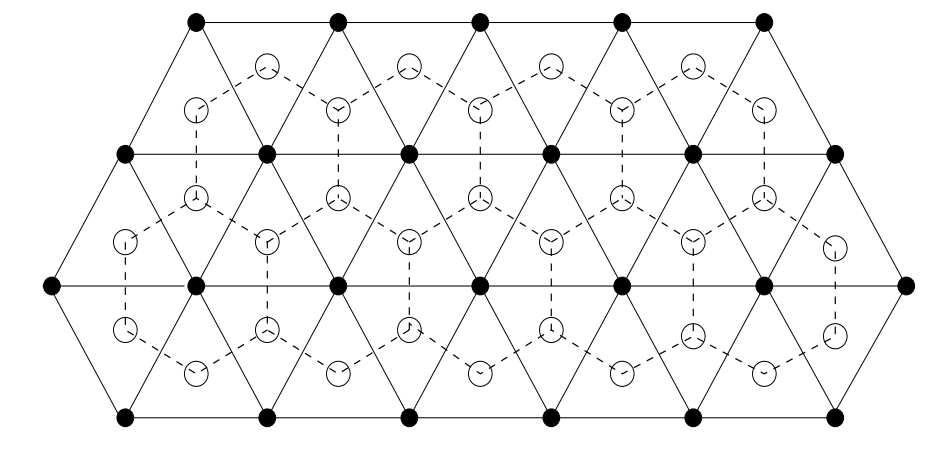
\includegraphics[width=0.85\linewidth]{part4/dualTriag.png}}
 	\caption{Дуальные друг к другу решетки: треугольная и гексагональная решетки~\cite{mussardo2010}}
 	\label{dualTriag}
 \end{figure}

\subsection{Гексагональная решетка}

Для получения гексагональной решетки из обобщенной квадратной решетки необходимо приравнять любое из четырех обменных взаимодействий нулю. Получим решетку типа «кирпичная кладка», которая в свою очередь топологически эквивалентна гексагональной решетке (рисунок \ref{toHex}).

Точное решение для гексагональной решетки так же может быть получено комбинаторным методом Вдовиченко--Фейнмана. Матрица коэффициентов $\Lambda$ для гексагональной решетки имеет следующий вид
\begin{multline}
\Lambda (p, q, \mu\; |\; p, q, \mu^{'}) = \\ =
\begin{pmatrix}
0 & 0  & 0  & x \alpha^{-1} \epsilon^{-p}  & 0  & z \alpha \epsilon^{p+q} \\
0 & 0  & 0  & x \alpha \epsilon^{-p}  & y \alpha^{-1} \epsilon^{-q}  & 0 \\
0 & 0  & 0  & 0  & y \alpha \epsilon^{-q}  & z \alpha^{-1} \epsilon^{p+q} \\
y \alpha \epsilon^{q} & z \alpha^{-1} \epsilon^{-p-q}  & 0  & 0  & 0  & 0 \\
0 & z \alpha \epsilon^{-p-q}  & x \alpha^{-1} \epsilon^p  & 0  & 0  & 0 \\
y \alpha^{-1} \epsilon^{q} & 0  & x \alpha \epsilon^p  & 0  & 0  & 0 
\end{pmatrix},
\end{multline}
где $x = \th K_1$, $y = \th K_2$, $z = \th K_3$, $\epsilon = e^{2\pi i/L}$ и $\alpha = e^{i\pi/6}$.

Производя соответствующие расчеты, получаем точное аналитическое решение модели Изинга на гексагональной решетке~\cite{houtapell1950}
\begin{multline}
\ln \frac{\lambda_h}{2} = \frac{1}{16 \pi^2} \int_{0}^{2\pi} \int_{0}^{2\pi} \ln \bigg[\frac{1}{2} \bigg( \ch 2K_1 \ch 2K_2 \ch 2K_3 + 1 \\ - \sh 2 K_1 \sh 2 K_3 \cos (\omega_1 - \omega_2)  - \sh 2 K_1 \sh 2 K_2 \cos \omega_1  - \\ - \sh 2 K_2 \sh 2 K_3 \cos \omega_2 \bigg) \bigg] d\omega_1 d\omega_2,
\end{multline}
где $K_1 = J_1/T$, $K_2 = J_2/T$, $K_3 = J_3/T$. 


Рассмотрим подлогарифмическое выражение при $J_1 = J_2 = J_3 = J$ и $\omega_1 = \omega_2 = 0$, тогда
\begin{equation}
\frac{1}{2}\bigg(\ch^3 \bigg(\frac{2J}{T_c} \bigg) + 1 - 3 \sh \bigg(\frac{2J}{T_c}\bigg)\bigg) = 0.
\label{lab1}
\end{equation}

Решив уравнение \eqref{lab1}, получим температуру перехода для гексагональной решетки
\begin{align}
T_c^{hex} &= \frac{2J}{\ln (2 + \sqrt{3})};& T_c^{hex} &= J \cdot 1.51865\dots.
\end{align}

Гексагональная решетка, как и квадратная решетка, не является фрустрированной при любых параметрах обменных взаимодействий в отсутствие магнитного поля. Таким образом, это значит, что на гексагональной решетке можно расположить спины так, чтобы каждая пара ближайших соседей была антипараллельна.

\subsection{Другие виды решеток}

При равенстве двух обменных взаимодействий нулю, реализуется случай обобщенной модели Изинга на одномерной цепочке, который был подробно исследован в Главе~\ref{ch:ch2}.

Если все взаимодействия, кроме одного, оказываются равными нулю, то задача сводится к случаю решетки димеров, так же рассмотренных в Главе~\ref{ch:ch2}.


\section{Выводы по главе}

Впервые выведенное с помощью комбинаторного метода Вдовиченко--Фейнмана точное выражение для свободной энергии Гельмгольца обобщенной модели Изинга на квадратной решетке с двумя трансляциями позволяет исследовать термодинамические и фрустрационные свойства данной решетки.

Результаты, описанные в этой главе, опубликованы автором в работах~\cite{confbib7, confbib8, scbib2}.

\FloatBarrier